\chapter{Photon Detection System}
\label{ch:fddp-pd}

%%%%%%%%%%%%%%%%%%%%%%%%%%%%%%%%%%%%%%%%%%%%%%%%%%%%%%%%%%%%%%%%%%%%
\section{Overview}
\label{sec:fddp-pd-1}

%%%%%%%%%%%%%%%%%%%%%%%%%%%%%%%%%
\subsection{Introduction}
\label{sec:fddp-pd-1.1}

This chapter describes the Photon Detection System (PDS) for the DUNE Dual-Phase (DP) Far Detector (FD). It is essential to ensure that the DP FD PDS is optimized for the full DUNE physics program. In particular, low energy signals like supernova (SN) neutrinos and multi-messenger astronomy, other low-energy signals, and proton decay, will have more stringent requirements on photon detector system performance than the primarily higher energy, beam-synchronous, neutrino oscillation physics. The final specifications of the system will be determined in order to achieve these physics requirements. This Technical Proposal chapter will concentrate on direct projection of the ProtoDUNE-DP design to the DUNE scale. The optimization and final design of the Dual-Phase Photon Detector (DPPD) system will be driven by the ProtoDUNE-DP \cite{protoDUNDP-tdr} data and simulation studies.


The chapter begins with an overview of the system in section~\ref{sec:fddp-pd-1}. Section~\ref{sec:fddp-pd-2} describes the photo-sensors, namely photomultiplier tubes (PMTs) and the related high-voltage system, wavelength shifters and light collectors. The mechanics associated with the PMTs is described in Section~\ref{sec:fddp-pd-3}, and the readout electronics in ~\ref{sec:fddp-pd-4}. Section~\ref{sec:fddp-pd-5} details the photon calibration system to monitor the PMT gain and stability. Then, the photon detector performance is described in Section~\ref{sec:fddp-pd-6}, and the operations in Section~\ref{sec:fddp-pd-7}. Interfaces with other subsystems are described in Section~\ref{sec:fddp-pd-8}. Section~\ref{sec:fddp-pd-9} includes the installation, integration and commissioning plans. Then, the quality control procedures are outlined in Section~\ref{sec:fddp-pd-10}. The main safety issues to consider are specified in Section~\ref{sec:fddp-pd-11}. To finish, the management and organization is described in Section~\ref{sec:fddp-pd-12}.

%%%%%%%%%%%%%%%%%%%%%%%%%%%%%%%%%
\subsection{Physics and the Role of Photodetection}
\label{sec:fddp-pd-1.2}

The main physics goals of the DUNE DP liquid argon (LAr) Time Projection Chamber (TPC) is to register beam events from LBNF at Fermilab, and operate outside of the beam spill as an efficient observatory for supernovae explosions and proton decays. DUNE will also collect atmospheric neutrino and muon events, and will conduct searches for a number of exotic phenomena postulated by extensions of the Standard Model.  Expected or searched for signals can range in energy from a few MeV to many GeV and have characteristic time duration and topological features that challenge the performance of large noble liquid TPCs. An essential and critical part of the LAr TPC is the PDS, sensitive to light produced by interactions in argon \cite{Cuesta:2017nrs}. In DP TPCs, the timing of prompt scintillation light (usually referred as S1 signal) in LAr is needed for time stamping of events and propagation of tracks in the detector. The extraction and amplification of drift electrons in the gas phase (usually referred to as S2 signal) yields information on the drift time and amount of ionization charge, thus supplementing information from the charge readout on the anode plane. The interplay between the charge and light from an event allows to achieve the pattern recognition and energy of interactions.

Ionizing radiation in liquid noble gases leads to the formation of excimers in either singlet or triplet states, which decay radiatively to the dissociative ground state with characteristic S1 fast and slow lifetimes (fast is about 6\,ns, slow is about 1.6 $\mu$s in LAr with the so-called second continuum emission spectrum peaked at the wavelength of 128$\pm$10\,nm). This prompt and relatively high-yield (about 40,000 photons per MeV) of 128\,nm scintillation light is exploited in LAr TPC to provide the absolute time ($t_0$) of the ionization signal collected at the anode, thereby providing the absolute value of the drift coordinate of fully contained events, as well as a prompt signal used for triggering purposes.

The secondary scintillation light S2 is produced in the gas phase of the detector when electrons, extracted form the liquid, are accelerated in the electric field between the liquid phase and the anode. The secondary scintillation in the argon gas (i.e. a vapor phase) is the luminescence in gas caused by accelerated electrons in the electric field and in the Large Electron Multiplier (LEM) anode through Townsend amplification. For a given argon gas density, the number of photons of this S2 signal is proportional to the number of electrons, the electric field, and the length of the drift path in gas covered by the electrons. In an extraction field of 2.5\,kV/cm in gas, one electron generates about 75 photons. The time stretch of S2 reflects the extraction time of original ionization in the liquid phase into the gas phase, thus for about 1\,kV/cm electric field, the time scale of S2 is of the order of hundreds of microseconds. The time between the occurrence of the primary scintillation light and the secondary scintillation light is equivalent to the drift time of the electrons from the ionization coordinate to the LAr surface.

The baseline design of the light collection system calls for 8-inch diameter cryogenic PMTs distributed uniformly on the floor of the cryostat and electrically shielded from the bottom cathode plane. The proposed density of PMTs and their arrangement follows the design of the ProtoDUNE-DP detector. On the other hand, modeling and simulations of light collection both for ProtoDUNE and the DUNE detectors are still ongoing. Therefore, even critical system parameters and their impact on the physics reach are still tentative. Results from the ProtoDUNE will provide the critical validation of simulations and will guide optimizations for the large DUNE detector.

%%%%%%%%%%%%%%%%%%%%%%%%%%%%%%%%%
\subsection{Technical Requirements}
\label{sec:fddp-pd-1.3}

Photomultipliers provide the sharpest time information of events in the LAr TPC and in the gas phase of the extraction stage. Due to necessary wavelength-shifting of photons from the argon luminescence and shadowing by the cathode plane, the efficiency of light detection is challenging and requires careful mechanical, electrical, and optical designs.

PMTs will be installed with the baseline density of 1 per 1\,m$^2$. In order to extend the PMT light sensitivity region to the LAr light emission wavelength of 128\,nm, a wavelength shifter has to be used. Therefore, in the baseline plan, the hemispherical windows of the PMTs will be evaporated with a thin layer of Tetra-Phenyl-Butadiene (TPB) \cite{tpb} for wavelength-shifting into the range suitable for R5912 PMT photocathode sensitivity \cite{hamamatsu-5912}. PMTs have to be rigidly anchored to the bottom of the cryostat. Different PMT densities and placements along the walls are also being considered in simulations. High voltage (HV)/signal cables will be routed along the cryostat walls to feedthroughs installed in the roof of the cryostat. Each PMT will be controlled individually so that its gain can be individually adjusted to match the front-end dynamic range and signal-to-noise ratio. 

The cathode plane is placed at a height of about 2\,m above the bottom of the cryostat, and the PMT plane will be distant enough from the cathode plane, taking into account the high electrical rigidity of the LAr phase. In order to protect the PMTs, the ground grid will be installed and placed at an identical potential as the PMT photocathode (0\,V). The PMTs will be powered to about 1.5-2.0\,kV such that the PMT gain is $\sim$10$^7$-10$^9$. DPPD Consortium is presently in contact with PMT manufacturers, including Hamamatsu Photonics in Japan \cite{hamamatsu}, Electron Tubes Limited in the US and UK \cite{electrontubeslim}, and HZC in China \cite{hzc}, to define optimal choice and configuration of PMTs satisfying our requirements, tentatively summarized in Table~\ref{tab:dppd_t_1_3}. These requirements will be reviewed based on the physics needs. For this, simulations and ProtoDUNE-DP results will be key.

\begin{dunetable}
[Summary of tentative requirements for the photon detection system of the DP LAr TPC.]
{|l|l|l| p{0.8\textwidth}}
{tab:dppd_t_1_3}
{Summary of tentative requirements for the PDS of the DP LAr TPC. The table assumes the baseline choice of the R5912-MOD2 photomultiplier manufactured by Hamamatsu Photonics \cite{hamamatsu-5912}.}
\footnotesize
%  & & \\
{\bf Feature}	& {\bf Goal}  	& {\bf Comment	}	\\
%  & & \\ 
 \toprowrule
%%%%%%%%%%%%%%%%%%%%%%%%%%%%%%%%%%%%%%%%%%%%%%%%%%%%
{\bf Optical} & & \\ \colhline
spectral response & 128\,nm 	& Wavelength shifters are required				\\
% $\lambda_{max}$&	420\,nm		& from the Hamamatsu data sheet 				\\
% QE			& 22\%@390\,nm	& from the Hamamatsu data sheet @25$^\circ$C	\\
% 				&				& (QE is desired to be as high as practical)		\\ 
% window		& borosilicate glass	& high transmission to the TPB emission $\gamma$'s\\ 
\colhline
% %	uniformity		&				&
%%%%%%%%%%%%%%%%%%%%%%%%%%%%%%%%%%%%%%%%%%%%%%%%%%%%
{\bf Electronic}	&			&										\\ \colhline
	gain			& $10^7-10^9$	& Nominal gain										\\ 
	dark count		& $< 4$\,kHz	& from the Hamamatsu data sheet @25$^\circ$C at nom. gain	\\
% 	rise time		& 4\,ns		& from the Hamamatsu data sheet 				\\
% 	PHD			& 2.5			& SPE peak-to-valley ratio	 taken				\\
% 				&			& (from the Hamamatsu data sheet) 				\\
% 	linearity		& 1 -- 500\,PE's& from CR muons in the $3\times1\times1m^3$ detector	\\
%	pre-pulsing 	&			& 										\\
%	after-pulsing	&			&										\\
% %%%%%%%%%%%%%%%%%%%%%%%%%%%%%%%%%%%%%%%%%%%%%%%%%%%%	
% \colhline		
%  	{\bf Readout}	&			&										\\ \hline
% 	max signal	& 500\,PE		& TBD by the front-end ASIC (into 50\,$\Omega$)	\\
% 	noise		& 			&										\\
% 	ADC resolution & 12 bits		&										\\
%%%%%%%%%%%%%%%%%%%%%%%%%%%%%%%%%%%%%%%%%%%%%%%%%%%%
\colhline		
 	{\bf Electrical}	&			&									\\ \colhline
 	HV range		& $0 - 2000$\,V	& individual cable per each PMT			\\
	HV resolution	& 1\,V		&									\\
	HV jitter		& 100\,mV		&									\\
	HV noise		& 100\,mV		& noise from the power supply is one 		\\
				&			& of the contributors to the noise in 			\\
				&			& the signal lines. Filtering will be required 	\\
				&			& at the PMT base and at the signal splitter 	\\
				&			& to reduce this noise bellow the mV level.	\\
	HV grounding	& isolated		& the HV outputs shall be floating, 			\\
				&			& the crate ground is independent of  		\\
				&			& the return of the HV channels. 			\\ 
	isolation		& grid		& PMT's must be electrically shielded		\\
				&			& from the TPC cage						\\
	power		& $< 0.2$\,W/PMT& as low as possible is desired			\\
%	magnetics		& shielding	& desired								\\
%%%%%%%%%%%%%%%%%%%%%%%%%%%%%%%%%%%%%%%%%%%%%%%%%%%%	
\colhline			
      {\bf Mechanical} 	&			&									\\ \hline
      	cryogenics 	& 77\,K		& LAr will be operated at higher T, but		\\
				&			& PMT's must withstand tests in liquid nitrogen \\
	pressure 		& +2\,bar		& the argon column will be about 10\,m high	\\
\colhline			
\end{dunetable}
% \normalsize

% \begin{dunetable}
% [Summary of tentative requirements for the photon detection system of the DP LAr TPC.]
% {|l|l|l| p{0.8\textwidth}}
% {tab:dppd_t_1_3}
% {Summary of tentative requirements for the PDS of the DP LAr TPC. The table assumes the baseline choice of the R5912-MOD2 photomultiplier manufactured by Hamamatsu Photonics.}
% \footnotesize
% %  & & \\
% {\bf Feature}	& {\bf Goal}  	& {\bf Comment	}	\\
% %  & & \\ 
%  \toprowrule
% %%%%%%%%%%%%%%%%%%%%%%%%%%%%%%%%%%%%%%%%%%%%%%%%%%%%
% {\bf Optical} & & \\ \colhline
% spectral response & 300 -- 600\,nm 	& from the Hamamatsu data sheet 				\\
% $\lambda_{max}$&	420\,nm		& from the Hamamatsu data sheet 				\\
% QE			& 22\%@390\,nm	& from the Hamamatsu data sheet @25$^\circ$C	\\
% 				&				& (QE is desired to be as high as practical)		\\ 
% window		& borosilicate glass	& high transmission to the TPB emission $\gamma$'s\\ \colhline
% %	uniformity		&				&
% %%%%%%%%%%%%%%%%%%%%%%%%%%%%%%%%%%%%%%%%%%%%%%%%%%%%
% {\bf Electronic}	&			&										\\ \colhline
% 	gain			& $10^5-10^7$	&										\\ 
% 	dark count		& $< 4$\,kHz	& from the Hamamatsu data sheet @25$^\circ$C 	\\
% 	rise time		& 4\,ns		& from the Hamamatsu data sheet 				\\
% 	PHD			& 2.5			& SPE peak-to-valley ratio	 taken				\\
% 				&			& (from the Hamamatsu data sheet) 				\\
% 	linearity		& 1 -- 500\,PE's& from CR muons in the $3\times1\times1m^3$ detector	\\
% %	pre-pulsing 	&			& 										\\
% %	after-pulsing	&			&										\\
% %%%%%%%%%%%%%%%%%%%%%%%%%%%%%%%%%%%%%%%%%%%%%%%%%%%%	
% \colhline		
%  	{\bf Readout}	&			&										\\ \hline
% 	max signal	& 500\,PE		& TBD by the front-end ASIC (into 50\,$\Omega$)	\\
% 	noise		& 			&										\\
% 	ADC resolution & 12 bits		&										\\
% %%%%%%%%%%%%%%%%%%%%%%%%%%%%%%%%%%%%%%%%%%%%%%%%%%%%
% \colhline		
%  	{\bf Electrical}	&			&									\\ \colhline
%  	HV range		& $0 - 2000$\,V	& individual cable per each PMT			\\
% 	HV resolution	& 1\,V		&									\\
% 	HV jitter		& 100\,mV		&									\\
% 	HV noise		& 100\,mV		& noise from the power supply is one 		\\
% 				&			& of the contributors to the noise in 			\\
% 				&			& the signal lines. Filtering will be required 	\\
% 				&			& at the PMT base and at the signal splitter 	\\
% 				&			& to reduce this noise bellow the mV level.	\\
% 	HV grounding	& isolated		& the HV outputs shall be floating, 			\\
% 				&			& the crate ground is independent of  		\\
% 				&			& the return of the HV channels. 			\\ 
% 	isolation		& grid		& PMT's must be electrically shielded		\\
% 				&			& from the TPC cage						\\
% 	power		& $< 0.2$\,W/PMT& as low as possible is desired			\\
% 	magnetics		& shielding	& desired								\\
% %%%%%%%%%%%%%%%%%%%%%%%%%%%%%%%%%%%%%%%%%%%%%%%%%%%%	
% \colhline			
%       {\bf Mechanical} 	&			&									\\ \hline
%       	cryogenics 	& 77\,K		& LAr will be operated at this T		\\
% 				&			& PMT's must withstand tests in liquid nitrogen \\
% 	pressure 		& 2\,bar		& the argon column will be about 10\,m high	\\
% \colhline			
% \end{dunetable}
% % \normalsize


%%%%%%%%%%%%%%%%%%%%%%%%%%%%%%%%%
\subsection{Detector Layout}
\label{sec:fddp-pd-1.4}

The PMT plane will be placed below the cathode plane far enough to be sufficiently electrically shielded. According to the baseline plan, the PMTs will be uniformly distributed across this plane with a density of 1 PMT/m$^2$, with a total of 720 PMTs installed. Other PMT configurations as determined by the simulations are also being considered. The PMTs will be individually mounted to the cryostat floor. The exact location of the PMTs will be determined by the location of the other floor structures like the cryogenic piping. The outline of the DUNE-DP is shown in Fig. \ref{fig:dppd_3_1}.

\begin{dunefigure}[The DUNE DP detector (partially open) with cathode, PMTs, field cage and anode plane with chimneys.]{fig:dppd_3_1}
{The DUNE DP detector (partially open) with cathode, PMTs, field cage and anode plane with chimneys.}
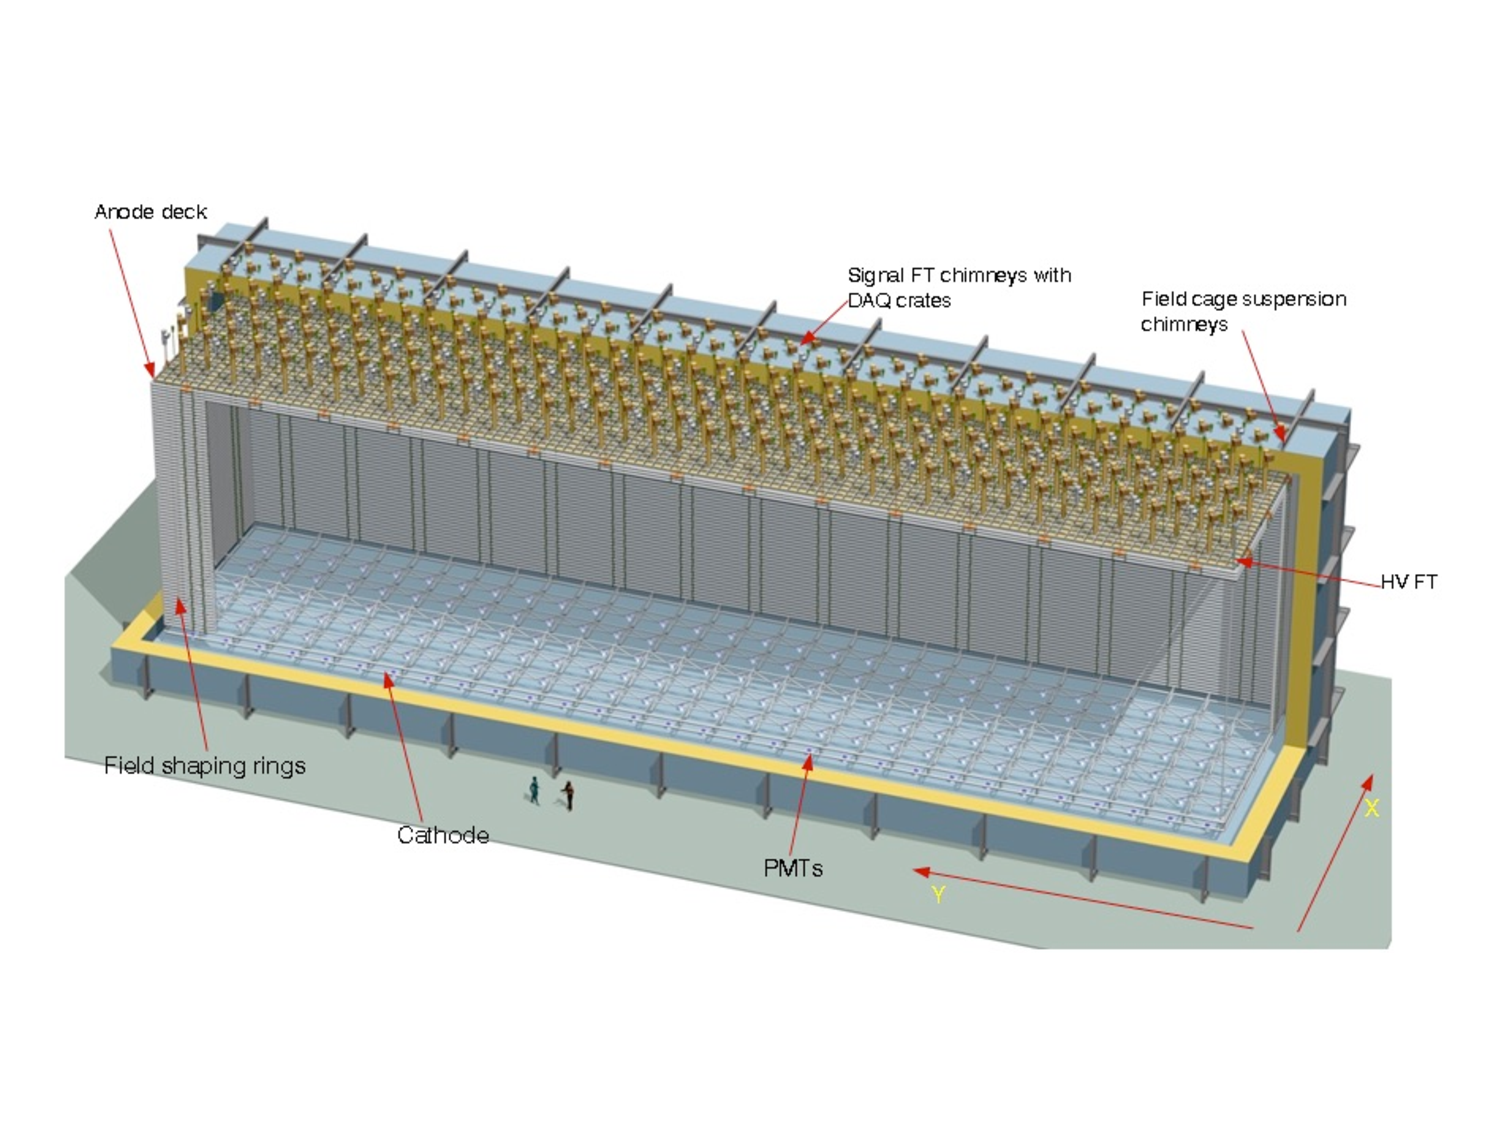
\includegraphics[width=0.8\textwidth]{dppd_3_1}
\end{dunefigure}

Since few light sensors are directly sensitive to 128\,nm a wavelength shifter will be required. TBP coating directly on the PMT is the default plan. Light collectors to increase the photons detected are under study. A single cable will be used per PMT to carry power and signal, and splitters will be placed out of the cryostat. A photon calibration system will be formed by external light sources and internal optical fibers.  

The cable trays from the side walls of the cryostat to the PMTs will carry the cables and calibration fibers. The cables and fibers will be routed from the feedthrough flanges at the top of the cryostat and  combined at the side wall trays. These side trays will carry the HV/signal cables in blocks of 24 PMTs and four calibration fibers. Therefore, each block of 24 PMTs in a 6$\times$4 $m^2$ area will form a sector of underground installation totaling in 30 sectors.

% %%%%%%%%%%%%%%%%%%%%%%%%%%%%%%%%%
\subsection{Operation Principles}
\label{sec:fddp-pd-1.5}

The PDS can operate in different acquisition modes depending on the trigger. These modes will include:

\begin{itemize}
\item External trigger: this is mainly the case of the trigger generated by the beam, but also data with random trigger can be taken. 
\item PDS trigger: the PDS can provide the trigger for cosmic ray events, SN burst, etc.
\item Continuous mode: acquisition in continuous mode is also foreseen.
\item Calibration: during PDS calibrations, the trigger will be provided by the light source used to calibrate.
\end{itemize}

Then, the signal readout system will extract from the PMT signals S1 and S2 shape, charge, and timing. The photon calibration system will determine the PMT gain, measuring the single photoelectron spectrum, and study the stability.  


%A charged particle crossing the LAr will ionize the argon and produce at the same time primary scintillation light of 128 nm. More detailed description of the light production with visuals can be found in Section \ref{sec:fddp-pd-6}. Within the TPC, the detection of these photons allows to trigger the event and thus, in combination with the arrival time of the drift electrons at the charge readout plane, the determination of the distance of the event to the anode plane. The knowledge of this drift distance allows to apply corrections for the electron attachment in the liquid due to impurities. Since few light sensors are directly sensitive to 128 nm, the detector approach foresees to convert the 128 nm photons by the use of suitable wavelength shifting material into photons of 460 nm. Large photomultipliers can be used to detect these photons allowing to cover large areas at a reasonable cost. The PMT signals provide information about the time of the event, the amount of light produced in the event and the geometrical distribution of the light. Measuring these information allows to define trigger criteria to select the relevant physics events for data recording.  

%%%%%%%%%%%%%%%%%%%%%%%%%%%%%%%%%%%%%%%%%%%%%%%%%%%%%%%%%%%%%%%%%%%%
\section{Photosensor System}
\label{sec:fddp-pd-2}

%%%%%%%%%%%%%%%%%%%%%%%%%%%%%%%%%
\subsection{Photodetector Selection and Procurement}
\label{sec:fddp-pd-2.1}

The photodetector selected as baseline for the light-readout system is the Hamamatsu R5912-MOD2 PMT as used in ProtoDUNE-DP. The Hamamatsu R5912-MOD2, see Figure \ref{fig:dppd_2_1}, is an 8-inch, 14-stage, high gain PMT (nominal gain of 10$^9$). In addition, this PMT was designed to work at cryogenic temperature adding a thin platinum layer between the photocathode and the borosilicate glass envelope to preserve the conductance of the photocathode at low temperature. This particular PMT has proven reliability on other cryogenic detectors. The same or similar PMTs have been successfully operated in other LAr experiments like MicroBooNE \cite{microboone}, MiniCLEAN \cite{miniclean}, ArDMm, Icarus T600 \cite{icarus} and also in ProtoDUNE-DP \cite{protoDUNDP-tdr}. Contacts with other manufacturers such as Electron Tubes Limited (UK) \cite{electrontubeslim} and HZC (China) \cite{hzc} are on-going to engage them in the program.

\begin{dunefigure}[Picture of the Hamamatsu R5912-MOD2 PMT.]{fig:dppd_2_1}
{Picture of the Hamamatsu R5912-MOD2 PMT \cite{hamamatsu-5912}.}
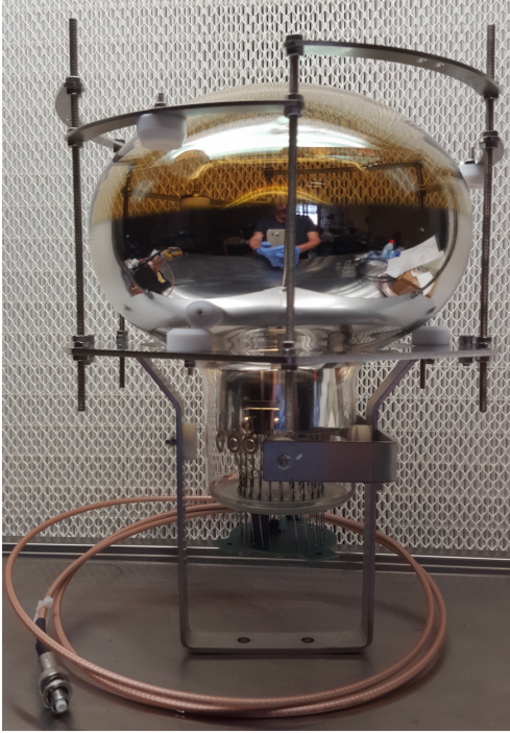
\includegraphics[width=0.2\textwidth]{dppd_2_1}
\end{dunefigure}

As the baseline number of PMTs, 720 + 80 spares, is high and several operations and tests have to be performed with them before the installation. To execute this plan, the PMTs have to be ordered with some time in advance. The envisioned operations are: assembly of the voltage divider circuit, mounting on the support structure, test at room and cryogenic temperatures, application of TPB coating, packing and shipment. And finally, they have to be re-tested on-site before installation (see Sections \ref{sec:fddp-pd-9} and \ref{sec:fddp-pd-10}). Considering the large number of PMTs required by DPPD, the purchase order has to be sent, at least, two years in advance of installation. The order should be staged to achieve a steady supply of PMTs for these installation processes. 

%%%%%%%%%%%%%%%%%%%%%%%%%%%%%%%%%
\subsection{Photodetector Characterization}
\label{sec:fddp-pd-2.2}

Before the installation, the most important parameters of the PMT response have to be measured with two aims: first, to reject under-performing PMTs and second, to store the characterization information in a database for later use during the detector commissioning and operation.

Basic and most important parameters to characterize are the dark counts rate vs voltage and the gain vs voltage. Both parameters must be measured at room and at cryogenic temperatures.

From the mechanical point of view, the test setup will require a light tight vessel that could be filled with a cryogenic liquid (argon or nitrogen) plus the infrastructure for filling and operating the vessel with temperature and liquid level controls. For ProtoDUNE-DP, 10 PMTs were tested at a time during a week, as the tests of the PMTs on cryogenics require several days for the PMT thermalization. Figure \ref{fig:dppd_2_2a} shows the PMTs being installed in the testing vessel used for the ProtoDUNE-DP PMTs. Increasing the capacity of the vessel, and thus the number of PMTs tested at a time, will reduce the characterization test duration.

\begin{dunefigure}[Picture of the PMTs being installed in the testing vessel used for the ProtoDUNE-DP PMTs]{fig:dppd_2_2a}
{Picture of the PMTs being installed in the testing vessel used for the ProtoDUNE-DP PMTs.}
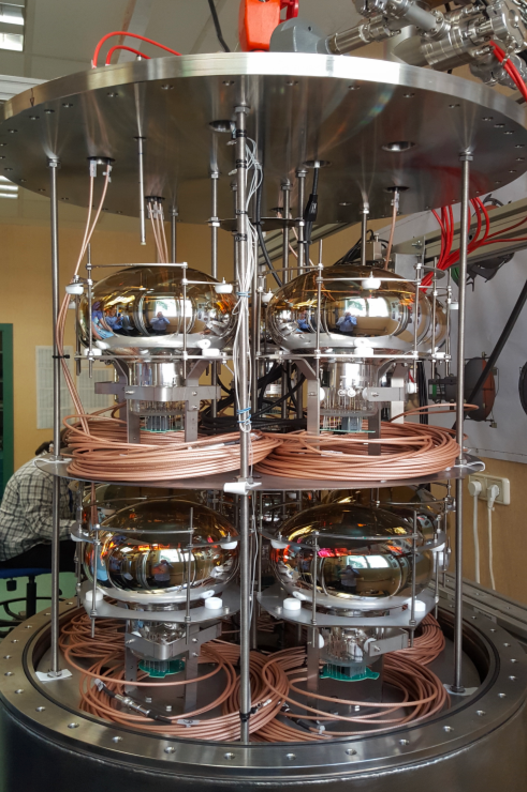
\includegraphics[width=0.3\textwidth]{dppd_2_2a}
\end{dunefigure}

Figure \ref{fig:dppd_2_2b} shows the sketch of the envisaged setup for PMT characterization tests. From the electronics point of view, the test setup will require a HV power supply, a discriminator, a counter for the dark rate measurements, a pulsed light source, and a charge-to-digital or analog-to-digital converter for the PMT gain vs voltage measurements. All those instruments must allow computer control to automatize the data acquisition.

\begin{dunefigure}[Sketch of the setup for PMT characterization tests.]{fig:dppd_2_2b}
{Sketch of the setup for PMT characterization tests.}
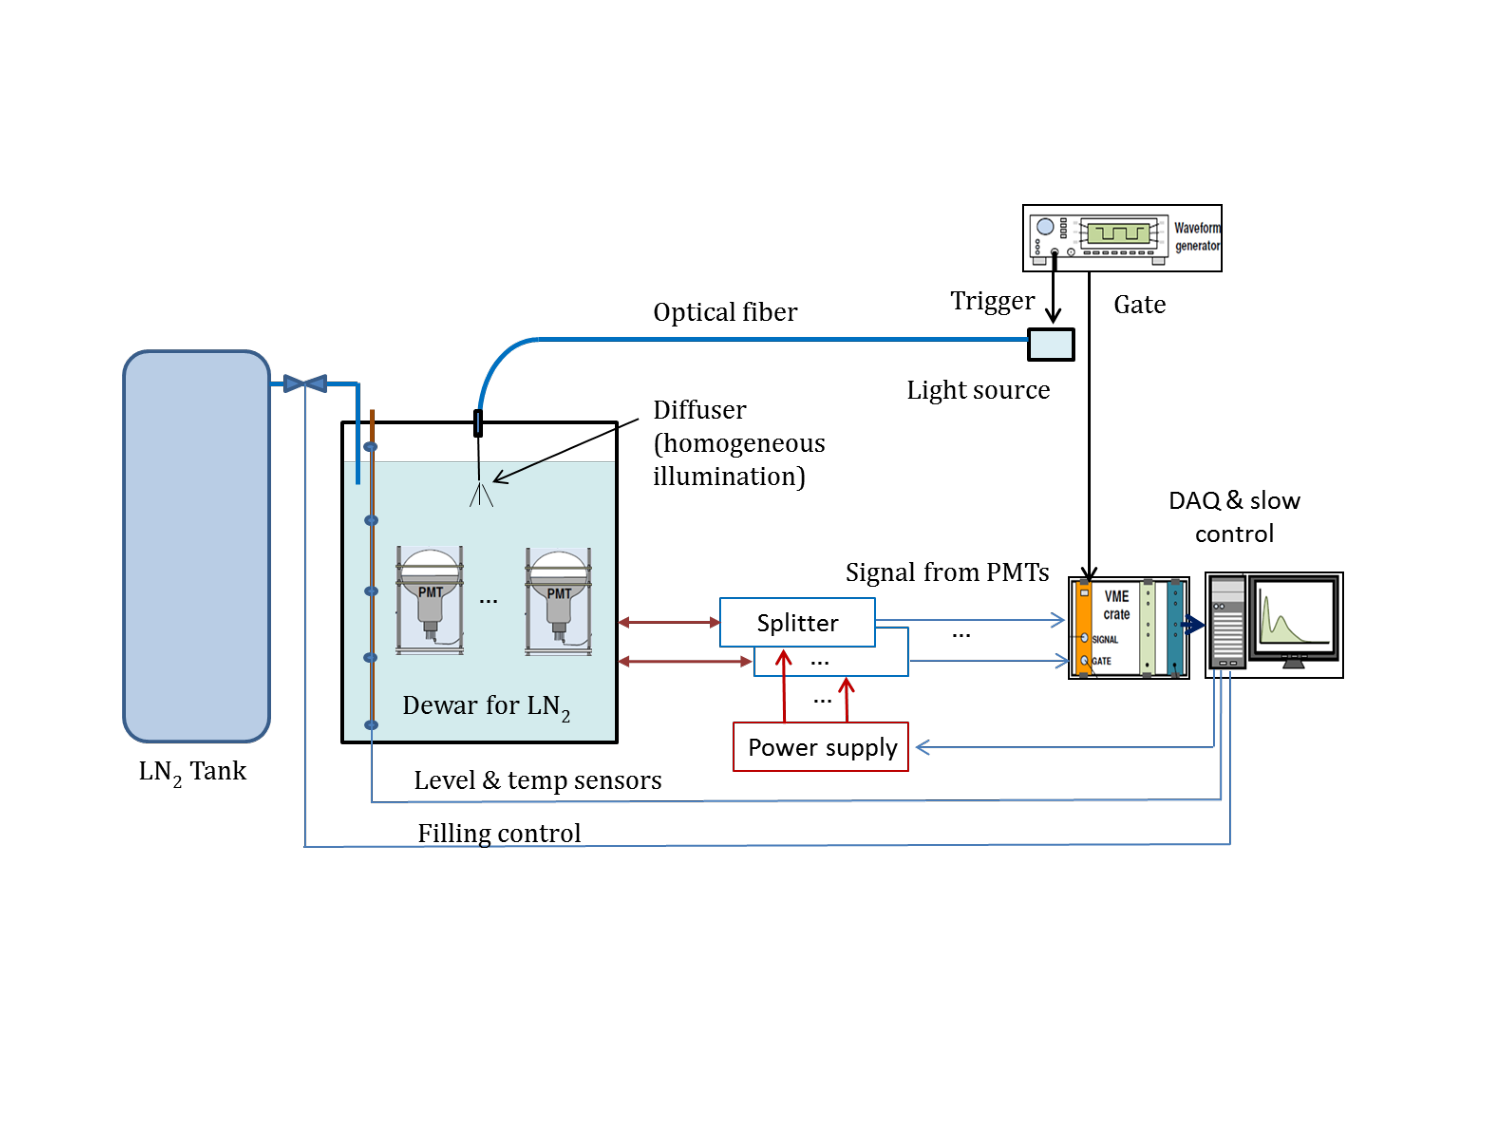
\includegraphics[width=0.8\textwidth]{dppd_2_2b}
\end{dunefigure}

%%%%%%%%%%%%%%%%%%%%%%%%%%%%%%%%%
\subsection{High Voltage System}
\label{sec:fddp-pd-2.3}

Based on the experience with the $3\times1\times1$\,m$^3$ DP prototype, for the PMT HV system, the A7030 power supply modules from CAEN \cite{caen-a7030} were chosen as baseline design. These modules provide up to 3\,kV with a maximal output current of 1\,mA and a common floating ground to minimize the noise. Module versions with 12, 24, 36 or 48 HV channels are available. The HV polarity can be chosen for each module. According to the baseline PMT powering scheme, modules with positive HV polarity will be acquired for the experiment. Modules with 48 HV channels and Radiall 52 connector are considered. The corresponding HV cable will connect the modules with the HV splitters which are described in Section \ref{sec:fddp-pd-4.2}. This choice will allow the design of a compact and most cost-effective system occupying between 1 and 2 racks only. For 720 PMTs, 15 A7030 modules (+ 2 spares) will be needed. These 15 HV modules will be installed in mainframes from CAEN.

For the type of HV cables between HV splitters and feedthroughs, the HTC 50-3-2 \cite{htc-50-3-2} have been chosen as baseline. The HTC 50-3-2 has a similar attenuation length compared to the RG-303/U \cite{rg303} which will be used inside the cryostat, but for a factor of 8 to 10 lower cost. These cables will be attached on one side directly to the HV splitter and will have an SHV connector on the other end.

Each PMT will be powered individually thus allowing the gain of all PMTs to be equalized by adjusting the operating voltage. A control software for this task will be provided taking into account the development of an interface to the PMT calibration system (Section \ref{sec:fddp-pd-5}) which will provide the calibration factors needed for the gain equalization.

%%%%%%%%%%%%%%%%%%%%%%%%%%%%%%%%%
\subsection{Wavelength Shifters}
\label{sec:fddp-pd-2.4}

The detector approach foresees to convert the 128 nm photons by the use of suitable wavelength shifting material into visible photons. The baseline plan is the already validated concept of coating the PMT windows with a thin film of TPB \cite{tpb}. TPB is a wavelength shifter with high efficiency for conversion of LAr scintillation VUV photons into visible light, where PMT cathode is sensitive. The TPB is deposited on the PMT by means of a thermal evaporator which consists of a vacuum chamber with two copper crucibles (Knudsen cells) placed at the bottom of the chamber. A PMT is fixed at the top of the evaporator, with its window pointing downwards, on a rotating support in order to ensure a uniform coating. The crucibles, filled with the TPB, are heated up to 220$^{\circ}$C. At this temperature, the TPB evaporates through a split in the crucible lid into the vacuum chamber, eventually reaching  the PMT window.

Several tests were performed in order to tune some parameters like the coating thickness (TPB surface density) and the deposition rate. For the tests, a PMT mock up covered with mylar foils has been used. A TPB density of 0.2 mg/cm$^2$ was chosen for ProtoDUNE-DP as this is the value where the PMT efficiency is stable as a function of the density. Efficiency measurements were performed using a VUV monochromator by comparing the cathode current of a coated PMT with the current value of a calibrated photodiode. As a result of the efficiency tests, about 0.8\,g of TPB must be placed in the crucibles at each evaporation, in order to achieve the desired PMT coating density. %The best deposition rate was fixed to about 6.5\,\AA/s. 
This value optimizes the quantity of TPB used per evaporation keeping, at the same, the coating density fluctuations below 5 $\%$. With these specifications, two to four PMTs can be coated per day at a single coating station. Then, a multiple coating stations will be required for timely operations.

%%%%%%%%%%%%%%%%%%%%%%%%%%%%%%%%%
\subsection{Light Collectors}
\label{sec:fddp-pd-2.5}

Although we are still lacking physics simulations that would include details and photon collection of large DUNE detectors, it can be generally argued that further optimization, or cost-effectiveness per physics reach, of light collection is desirable. Following many past examples of detectors that augmented their photodetectors with light collectors, we are considering incorporating such infrastructure into the DP detector.

In the case of LAr TPC, there are at least four main parameters for optimization: i) the number of PMTs per unit area, ii) the placement of PMTs to minimize interference with other components, iii) the augmentation of PMTs with additional light collectors, and iv) the choice of where and how the original 128\,nm photons can be wavelength-shifted. The most obvious direction for optimizing cost effectiveness are the latter two options. The option of shifter-reflectors that either include increasing the effective area of PMT windows or move shifting of light closer to the cathode and attaching wave-guides coupled to the PMTs are still under study.

%%%%%%%%%%%%%%%%%%%%%%%%%%%%%%%%%%%%%%%%%%%%%%%%%%%%%%%%%%%%%%%%%%%%
\section{Mechanics}
\label{sec:fddp-pd-3}

%%%%%%%%%%%%%%%%%%%%%%%%%%%%%%%%%
\subsection{Mechanical Structure of the Photosensor}
\label{sec:fddp-pd-3.1}

An individual PMT mount has been designed and tested in the WA105 $3\times1\times1$\,m$^3$ detector \cite{Zambelli:2017dkg}. The same design will be used for ProtoDUNE-DP and is foreseen for DUNE DP FD. The PMT mount was manufactured and assembled at CIEMAT for ProtoDUNE-DP and the WA105 $3\times1\times1$\,m$^3$ detector. A PMT with the mechanical structure is shown in Figure \ref{fig:dppd_2_1}. The support frame structure is mainly composed of 304L stainless steel with some small Teflon (PTFE) 6.6 pieces assembled by A4 stainless steel screws that minimize the mass while ensuring the PMT support to the cryostat membrane. The design was done taking into account the shrinking of the different materials during the cooling process to avoid the break of the PMT glass.

%%%%%%%%%%%%%%%%%%%%%%%%%%%%%%%%%
\subsection{Photosensor Fixation to the Membrane Floor}
\label{sec:fddp-pd-3.2}

A uniform array of 720 cryogenic Hamamatsu R5912-MOD2 PMTs, below the transparent cathode structure, will be fixed on the membrane floor in the areas between the membrane corrugations. The fixation is done via a stainless steel supporting base, that could be point glued to the membrane (glue: STYCAST 2850FT \cite{sytcast}, Material Safety Data-sheet). The arrangement of the PMTs will need to be optimized in order to be compatible with the presence of the cryogenic piping on the membrane floor, or any other element found in this area. Tests to ensure the correct performance under pressure will be carried out.

The mechanics for the attachment of the PMTs has been carefully studied for ProtoDUNE-DP. It must counteract the PMT buoyancy while avoiding stress to the PMT glass due to differentials in the thermal contraction between the support and the PMT itself. The weight of the support and photomultiplier overwhelms the buoyancy force of the system. Given the large standing surface of the stainless steel plate support basis, these supports will ensure as well stability against lateral forces possibly acting on the PMTs due to the liquid flow. Figure \ref{fig:dppd_3_2} depicts the PMT together with its support base attached to the bottom of the cryostat. %The calibration optical fiber that will be installed at each PMT in order to provide a homogeneous and configurable amount of calibration light is also visible in Fig.~\ref{fig:dppd_3_2}.

\begin{dunefigure}[Cryogenic Hamamatsu R5912-MOD2 photomultiplier fixed on the membrane floor.]{fig:dppd_3_2}
{Cryogenic Hamamatsu R5912-MOD2 photomultipliers fixed on the membrane floor, with the optical fiber of the calibration system.}
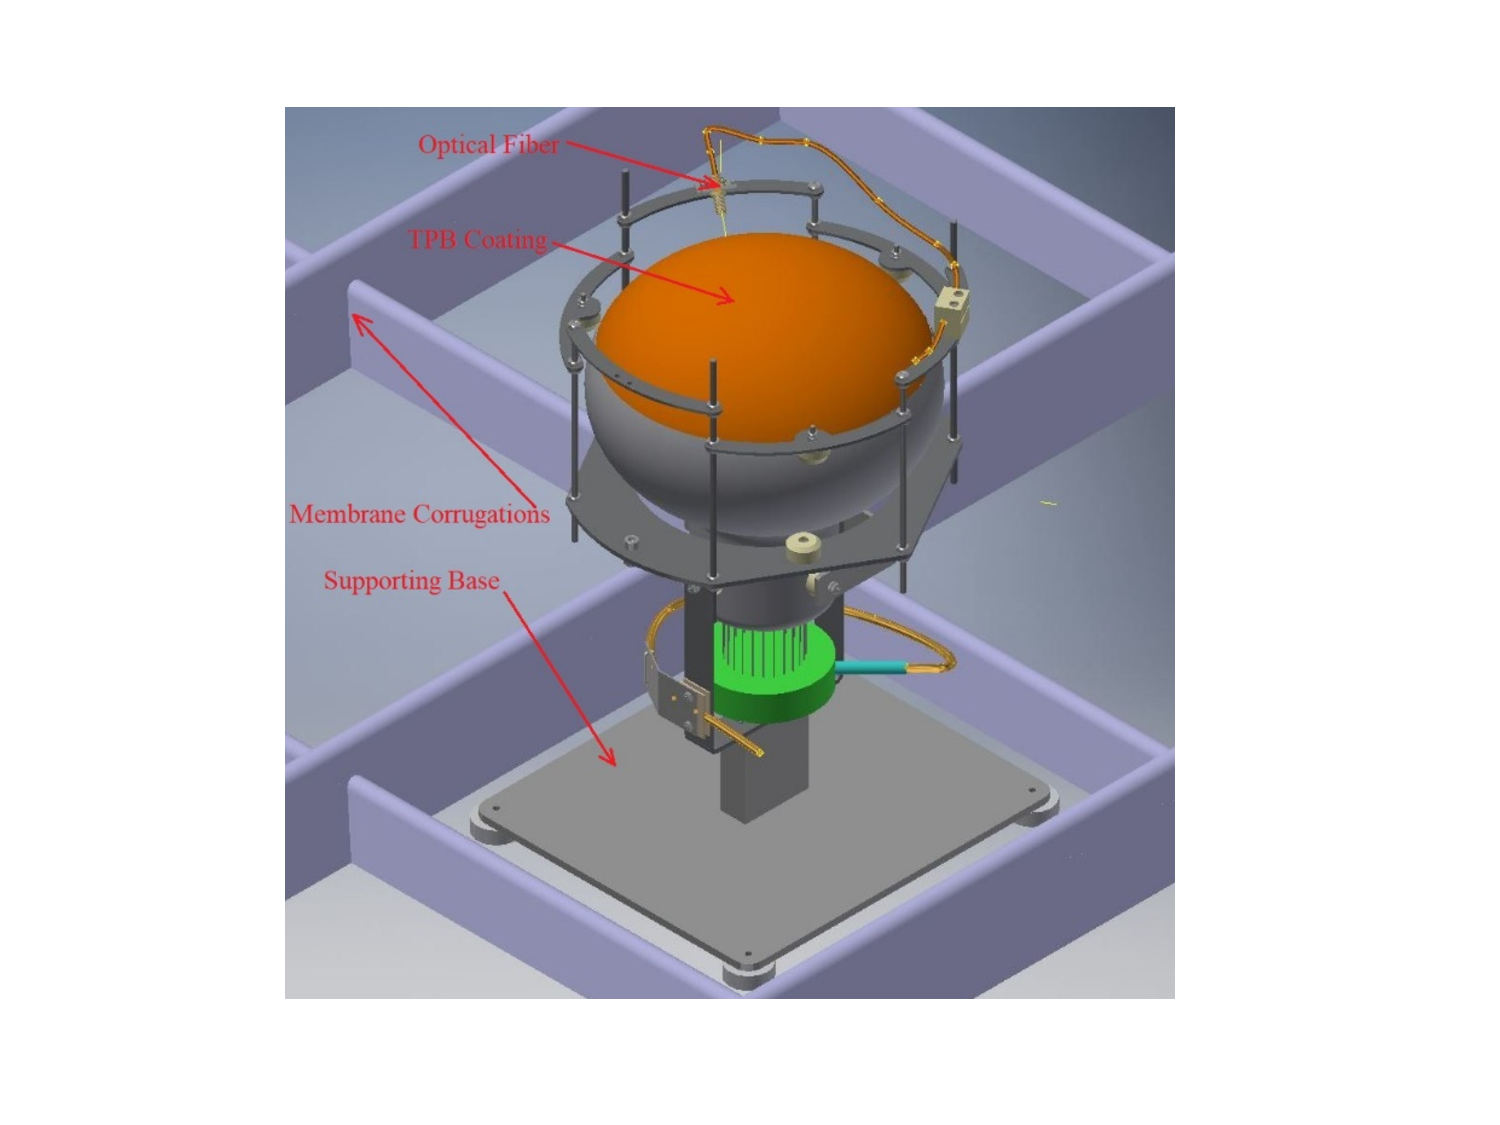
\includegraphics[width=0.5\textwidth]{dppd_3_2}
\end{dunefigure}

%%%%%%%%%%%%%%%%%%%%%%%%%%%%%%%%%%%%%%%%%%%%%%%%%%%%%%%%%%%%%%%%%%%%
\section{Readout Electronics}
\label{sec:fddp-pd-4}

%%%%%%%%%%%%%%%%%%%%%%%%%%%%%%%%%
\subsection{PMT High Voltage Dividers}
\label{sec:fddp-pd-4.1}

For the PMT power supply, the cathode grounding and positive high voltage applied to the anode was chosen for ProtoDUNE-DP, mainly, because a single cable is required for each PMT to carry power and signal. This configuration requires half of the cables and feedthroughs on the detector than the negative voltage configuration, which is a clear advantage since the number of PMTs in the detector is large. In addition, the cathode grounding shows less dark counts than the anode grounding scheme. The drawback is that a coupling capacitor must be used to separate the high voltage from the PMT signal, but, this signal and power splitting can be done externally from the detector. Figure \ref{fig:dppd_4_1} shows the positive power supply and cathode grounding scheme.

\begin{dunefigure}[Positive power supply and cathode grounding scheme.]{fig:dppd_4_1}
{Positive power supply and cathode grounding scheme.}
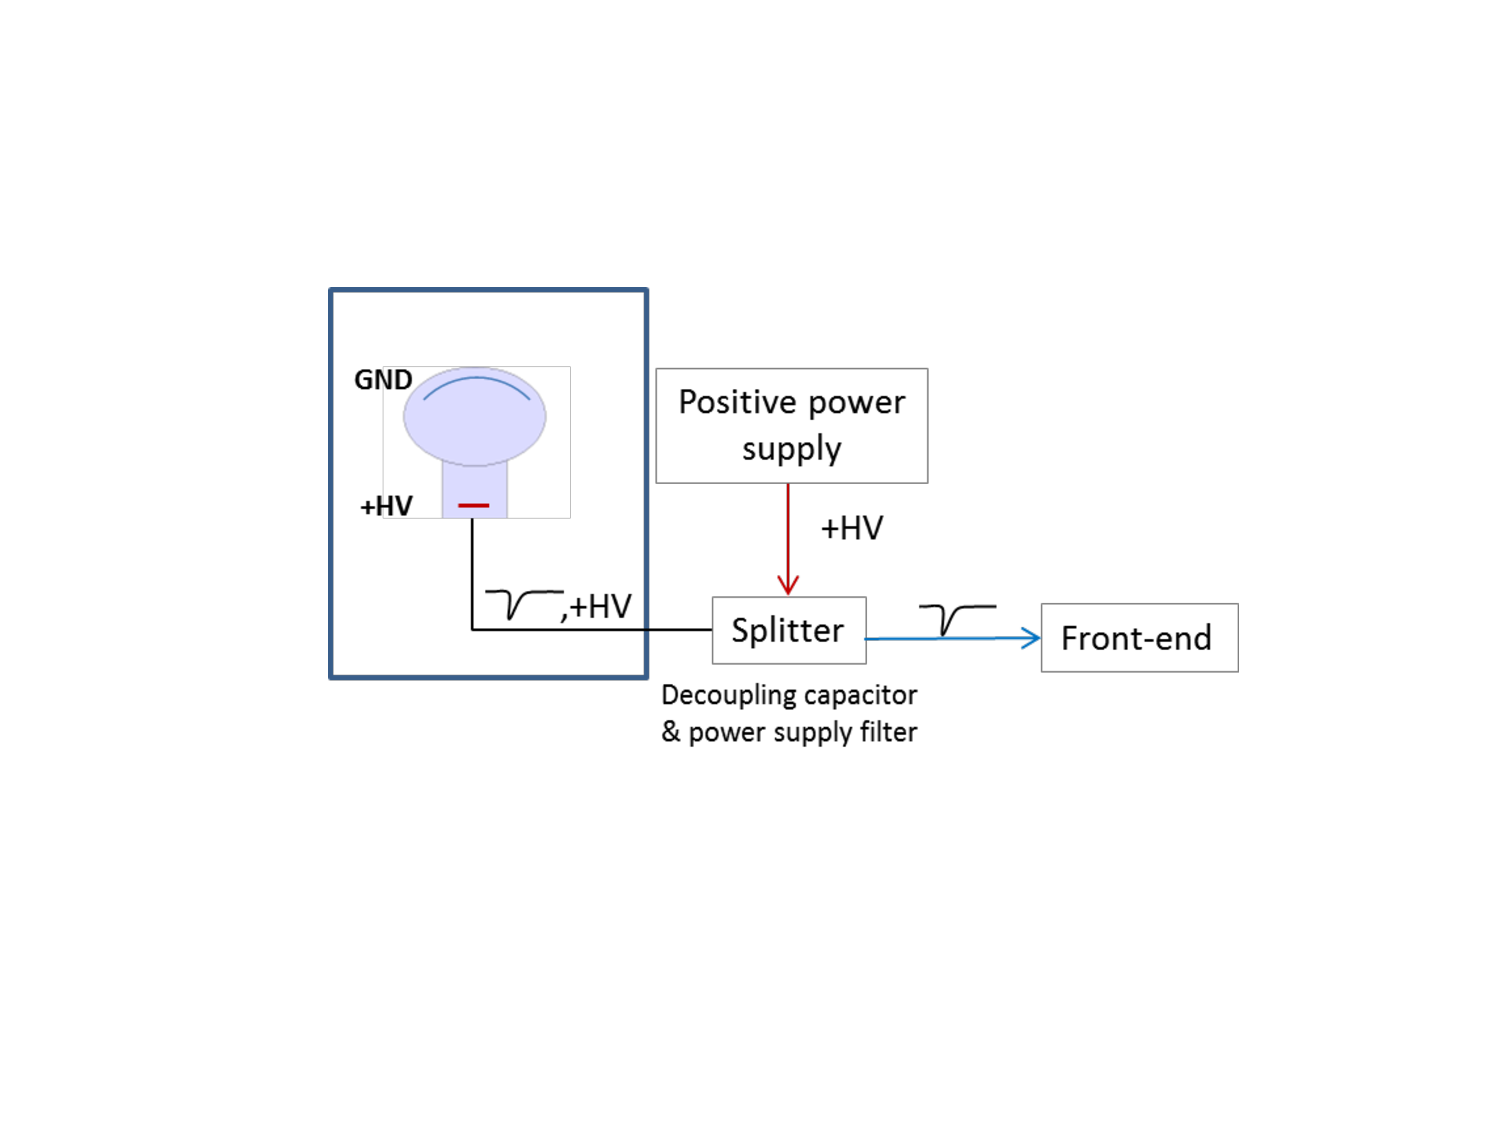
\includegraphics[width=0.5\textwidth]{dppd_4_1}
\end{dunefigure}

The PMT base circuit will be based only on resistors and capacitors as semiconductors do not work well in cryogenic temperatures. Nevertheless, the components will be carefully selected and tested to minimize the variations in their characteristics with temperature. The polarization current of the voltage divider (total circuit resistance) will be chosen to meet the PMT light linearity range and maximum power requirements.

%%%%%%%%%%%%%%%%%%%%%%%%%%%%%%%%%
\subsection{High Voltage/Signal Splitters}
\label{sec:fddp-pd-4.2}

HV/signal splitters will separate fast PMT response signal from the positive high voltage with capacitive decoupling. In addition, they will include a low pass filter between the HV supply and the PMT to reduce the noise.

Radiated electromagnetic interference (EMI) picked-up by the cables and conducted noise from the HV power supply can be synchronous across many PMT channels (coherent noise) that could be added-up producing false detector triggers. As the PMT signal can be as low as few mV, another important issue is the control of the EMI over the circuit. The EMI induced and conducted by the power supply cables will be reduced by the splitter HV input filter. To reduce the EMI directly received in the splitter circuit as well as the cross-talk between different splitter channels, each splitter channel will be enclosed into an individual metallic grounded box.

Figure \ref{fig:dppd_4_2} shows a generic splitter circuit where R1 and C1 form the HV input low pass filter (cut off frequency bellow 60 Hz). The resistor R7 and the LED have safety purpose only; warning when high voltage is applied to the splitter. C4 capacitor splits the signal coming from the PMT from the HV, and R2 prevents that the PMT signal goes to ground through the C1 capacitor. R4 and R5 are zero ohm optional resistors that allow some flexibility on the grounding configuration. Finally R3 ensures the discharging of C4 if the splitter is not connected to the 50 $\Omega$ input at the DAQ system.

\begin{dunefigure}[Generic splitter circuit diagram.]{fig:dppd_4_2}
{Generic splitter circuit diagram.}
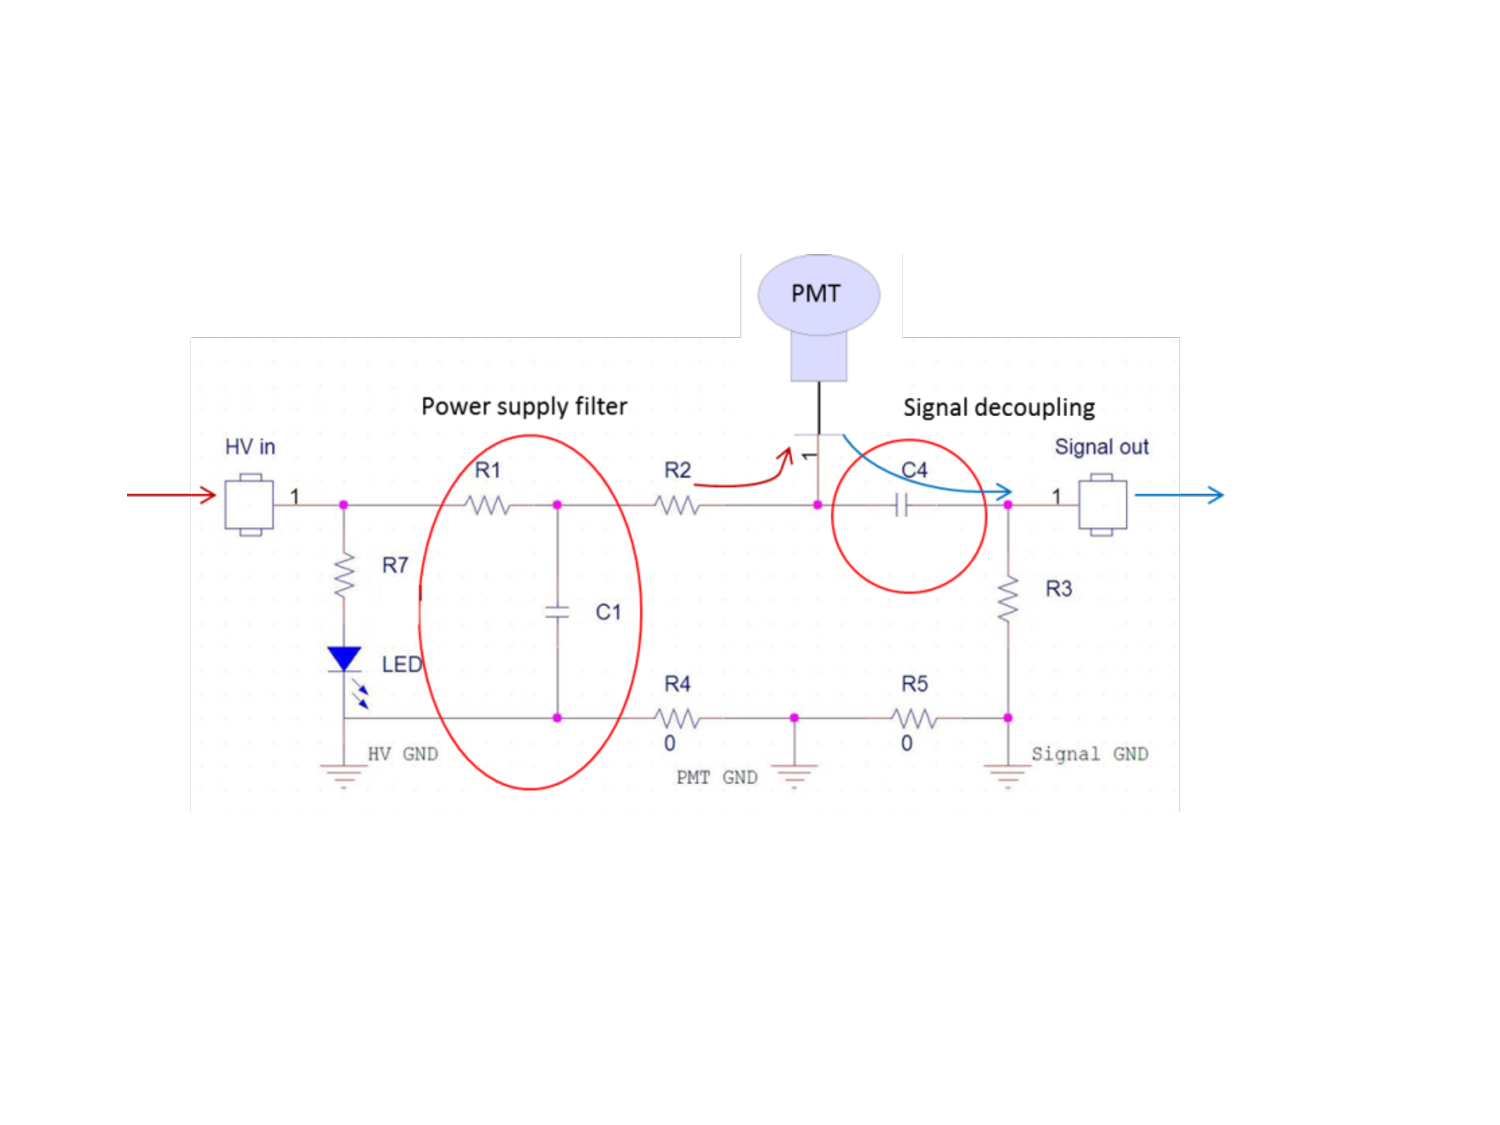
\includegraphics[width=0.7\textwidth]{dppd_4_2}
\end{dunefigure}

The RC constant of the capacitor C4 and the load (50 $\Omega$) must be as big as possible to minimize baseline oscillations due to the charge-discharge of the capacitor. Values of C4 between 150 nF and 300 nF have already been tested on the WA105 $3\times1\times1$\,m$^3$ prototype.

%%%%%%%%%%%%%%%%%%%%%%%%%%%%%%%%%
\subsection{Signal Readout Requirements}
\label{sec:fddp-pd-4.3}

We need to extract from the PMT signals:
\begin{itemize}
\item S1 fast component shape, charge and timing
\item S1 slow component amplitude and duration
\item S2 shape, charge and timing (distance from S1 and duration)
\item Single photoelectron (SPE) charge spectrum for gain calculation during PMT calibration
\item Trigger signal generation by the coincidence of several PMT signals
\end{itemize}

At this moment, we do not have an estimate of the dynamic range of the light that could reach the PMTs on the DUNE-DP far detector. %Also, the intensity range of light the PMT response needs to be linear is not determined. 
Our calculations are based on the signals detected by the PMTs on the WA105 $3\times1\times1$\,m$^3$ prototype. Although this prototype has a different dimension from the DUNE-DP detector, it is the only reference that we have for this estimates, until the ProtoDUNE-DP detector and simulations are operational.

In general, the PMT signal dynamic range goes from the mV level to several volts (over 50\,$\Omega$ load). During the operation of the WA105 $3\times1\times1$\,m$^3$ prototype, PMT signals larger than 2\,V were observed with PMT gains around 10$^6$. Figure \ref{fig:dppd_4_3_ab} shows the SPE waveforms (left, normalized) and amplitudes (right) for the $3\times1\times1$\,m$^3$ prototype at different voltages. The light levels in the DUNE-DP detector will have a larger dynamic range due to its large volume, so, higher gains will be required to see the far light signals. But, higher gains will make closer light signals to produce larger outputs, so, it is also essential that the front-end electronics can cover a large range of input voltages. To cover a dynamic range of 10\,V with a resolution below the mV level, 14 bits will be necessary (LSB $\sim$0.6\,mV). For 2\,V of dynamic range 12 bits would be sufficient (LSB $\sim$0.5\,mV). To finalize the required dynamic range, results from ProtoDUNE-DP and relevant simulations are needed.

\begin{dunefigure}[SPE waveforms and amplitudes from $3\times1\times1$\,m$^3$ prototype at different voltages.]{fig:dppd_4_3_ab}
{SPE waveforms (left) (normalized for comparison) and amplitudes (right) from $3\times1\times1$\,m$^3$ prototype at different voltages.}
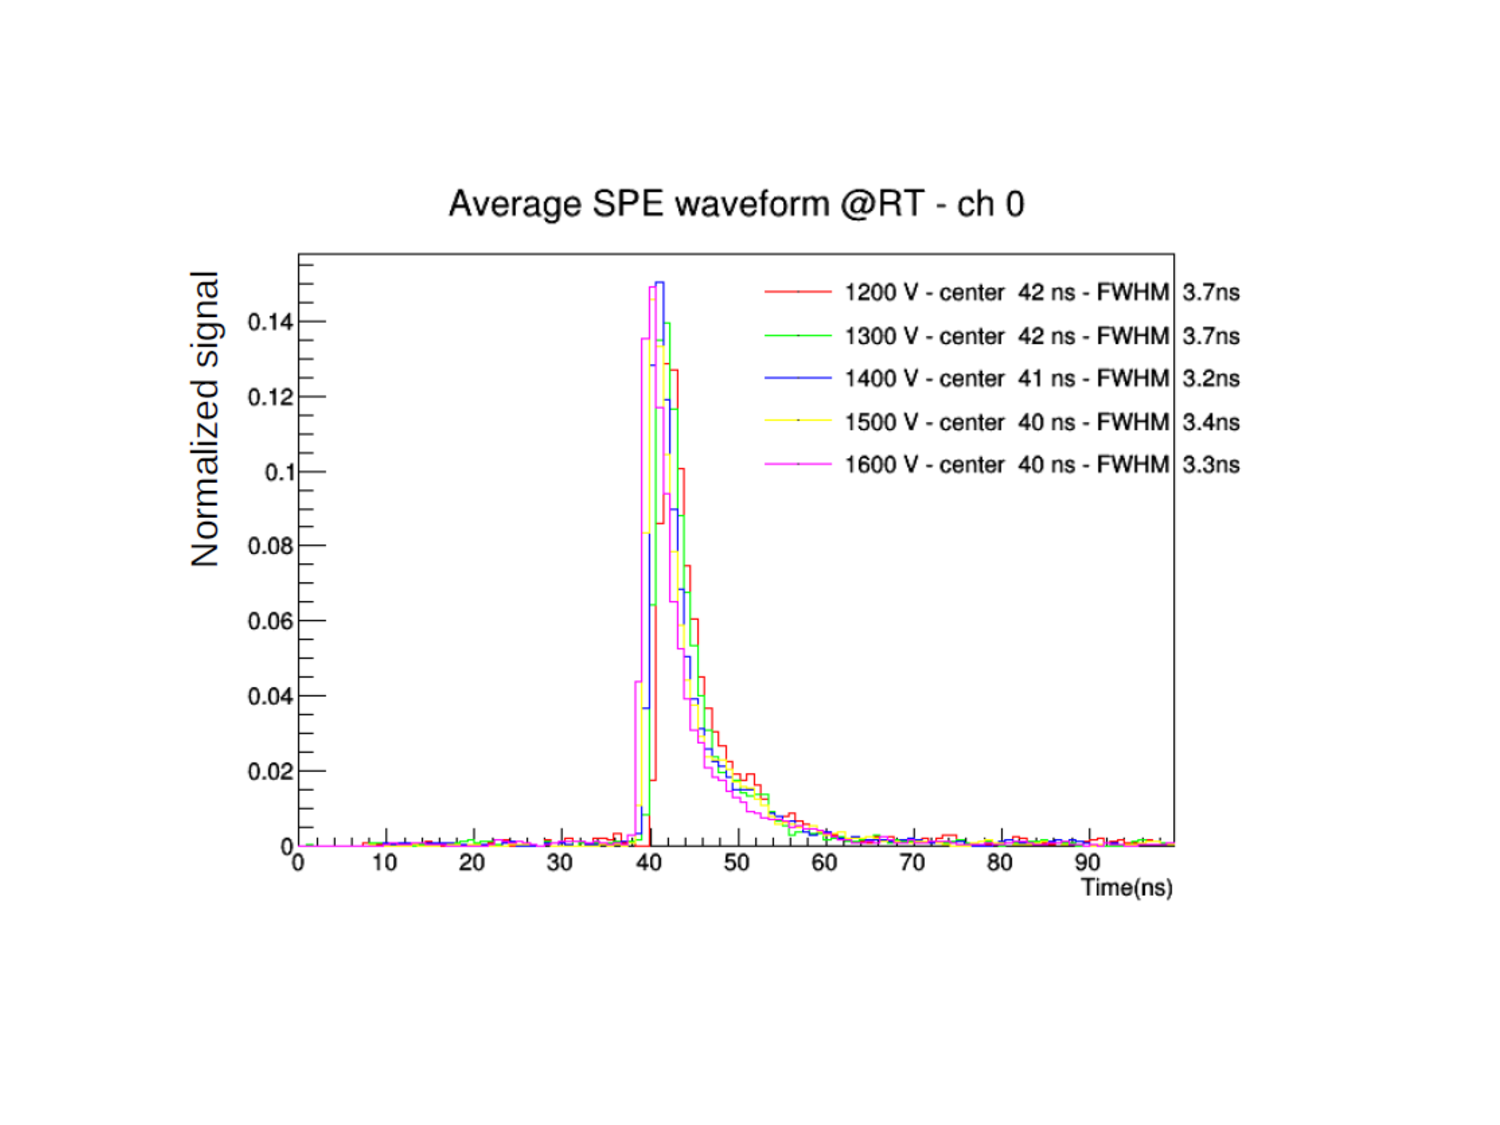
\includegraphics[width=0.45\textwidth]{dppd_4_3_a}
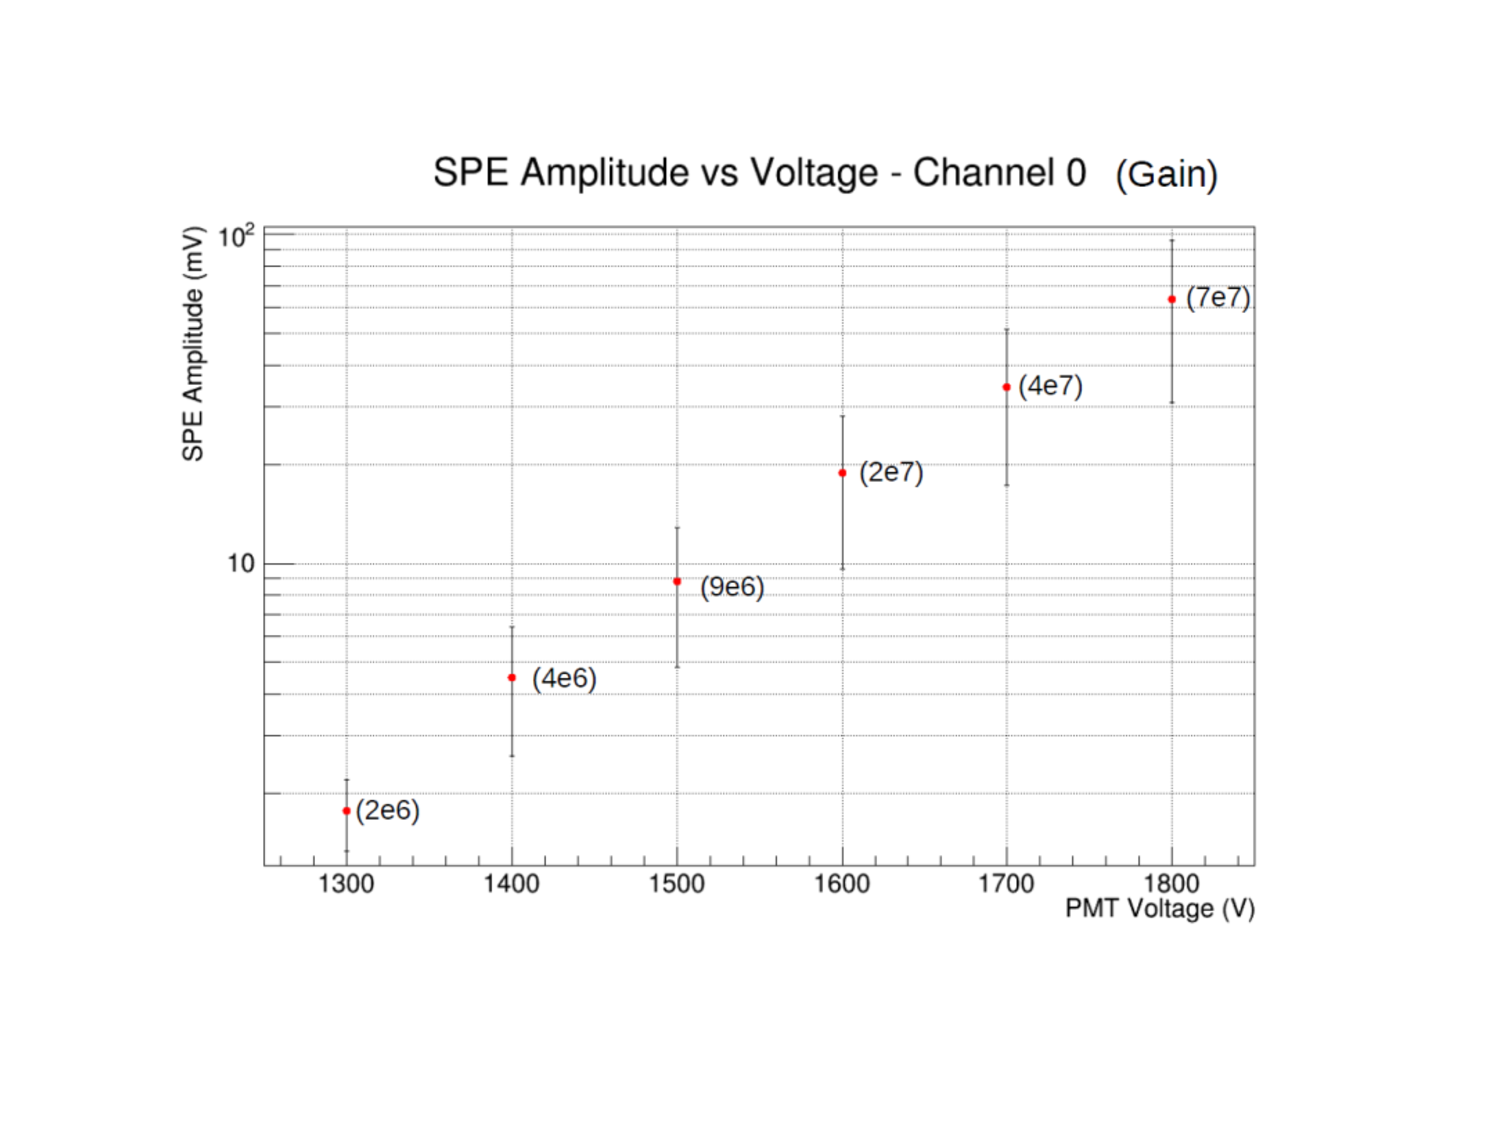
\includegraphics[width=0.45\textwidth]{dppd_4_3_b}
\end{dunefigure}

To calculate the PMT gains, the SPE charge measurement will be performed. Depending on the PMT gain, the SPE amplitude varies from the mV level to hundreds of mV. Due to the very long cables from the PMTs to the front-end electronics, the noise into the cables could be high. If one considers a noise level around 1\,mV,  the PMT gain must be set to 10$^6$ or higher in order to distinguish the SPE from noise. The average SPE pulse width is around 3.5\,ns full width at half maximum (FWHM). In order to digitize this signal to reconstruct it with fidelity, a sampling period of 1\,ns is required. %If this signal is only needed for charge calculation, the sampling frequency can be lower provided that the signal is previously low-pass filtered (Nyquist frequency).

The sampling frequency also affects the time tagging precision. The time uncertainty due to the PMT alone is around 3\,ns (transit time spread), there will be other factors, e.g. Rayleigh scattering, that will increase this uncertainty. The sampling period will also increase this uncertainty, so, the lower sampling frequency is the better. At the WA105 $3\times1\times1$\,m$^3$ prototype 4\,ns sampling was used  to digitize waveforms. 

The rate of the events observed on the WA105 $3\times1\times1$\,m$^3$ prototype was around 300\,kHz with the threshold at the SPE level. The rate at the DUNE FP, much bigger although placed underground is not know yet, but the time tagging system should be able to process events at high rates to assure that no events are lost. Figure \ref{fig:dppd_4_3_c} shows the event rates for different trigger thresholds observed with the $3\times1\times1$\,m$^3$ prototype.

\begin{dunefigure}[Event rates for different trigger thresholds observed on the WA105 $3\times1\times1$\,m$^3$ prototype.]{fig:dppd_4_3_c}
{Event rates for different trigger thresholds observed on the $3\times1\times1$\,m$^3$ prototype.}
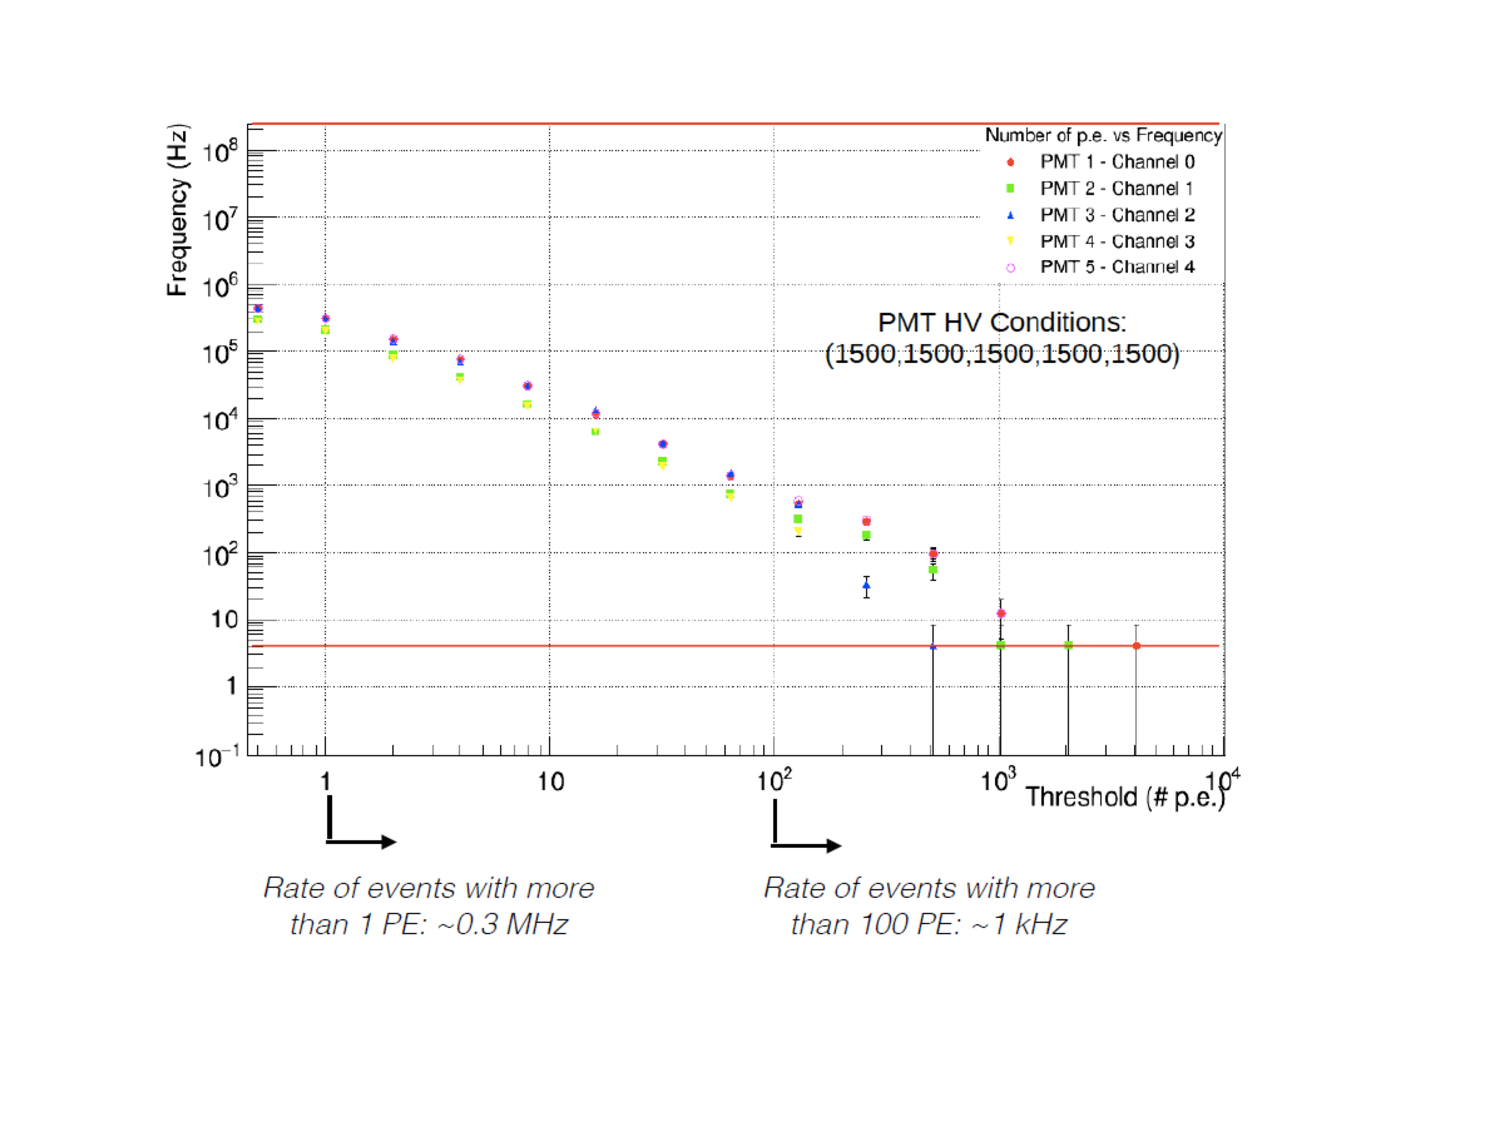
\includegraphics[width=0.5\textwidth]{dppd_4_3_c}
\end{dunefigure}

\textbf{Trigger generation:} For the same light event, the PMT signals will arrive to the front end electronics with different time delays that depend on different factors e.g. distance from the light emission point to the PMT, scattering and PMT transit time spread. In order to determine if there has been a coincidence on the signals from several PMTs, it is necessary to open a temporal coincidence window every time a signal from a PMT is received. The length of this window, the signal threshold level and the concrete PMTs contributing to this coincidence decision will be configurable by DAQ. Further information can be found in Section \ref{sec:fddp-pd-7.2}.

\textbf{DAQ Synchronization:} All the DAQ electronics will be in sync using White Rabbit protocol. A dedicated White Rabbit $\mu$TCA \cite{utca} slave node will be on the light read-out front-end electronics as sync receiver, distributing clocks to the different front-end cards.

%%%%%%%%%%%%%%%%%%%%%%%%%%%%%%%%%%%%%%%%%%%%%%%%%%%%%%%%%%%%%%%%%%%%
\section{Photon Calibration System}
\label{sec:fddp-pd-5}

%%%%%%%%%%%%%%%%%%%%%%%%%%%%%%%%%
\subsection{System Design and Procurement}
\label{sec:fddp-pd-5.1}

A photon calibration system integrated in DUNE DP far detector is required to monitor the calibration of the PMTs installed inside the LAr volume. The goal is to determine the PMT gain and maintain the PMT performance stability. A similar design as the one used in ProtoDUNE-DP will be used although some R\&D measurements are planed to make it more effective, reduce the cost and mitigate issues related to the scaling.

In ProtoDUNE-DP, an optical fiber will be installed at each PMT in order to provide a configurable amount of light (see Fig.~\ref{fig:dppd_3_2}). The calibration light will be provided by a blue LED of 460\,nm using a Kapuschinski circuit as LED driver which reduces significantly the cost of using a laser. There will be one LED connected to one fiber going to one female optical feedthrough from Allectra \cite{allectra}. In total,  there will be six LEDs placed in a hexagonal geometry. The direct light will go to the fiber, and the stray light to a SiPM used as reference sensor, being a single reference sensor in the center. Fibers of length 22.5-m (from Thorlabs $\phi$ 800-$\mu$m, FT800UMT \cite{ft800umt}, and stainless-steel jacket) will be used inside the cryostat. Each one of these fibers will be attached to a 1-to-7 fiber bundle (from Thorlabs $\phi$ 200-$\mu$m, FT200UMT \cite{ft200umt}, stainless-steel jacket common end, and black jacket at split ends), so that one fiber is finally installed at each PMT. A diagram of the ProtoDUNE-DP photon calibration system is shown in Figure \ref{fig:dppd_5_1}. Several tests to quantify the light losses of this design were performed successfully. 

\begin{dunefigure}[Diagram of the photon calibration system to be implemented in ProtoDUNE-DP.]{fig:dppd_5_1}
{Diagram of the photon calibration system to be implemented in ProtoDUNE-DP}
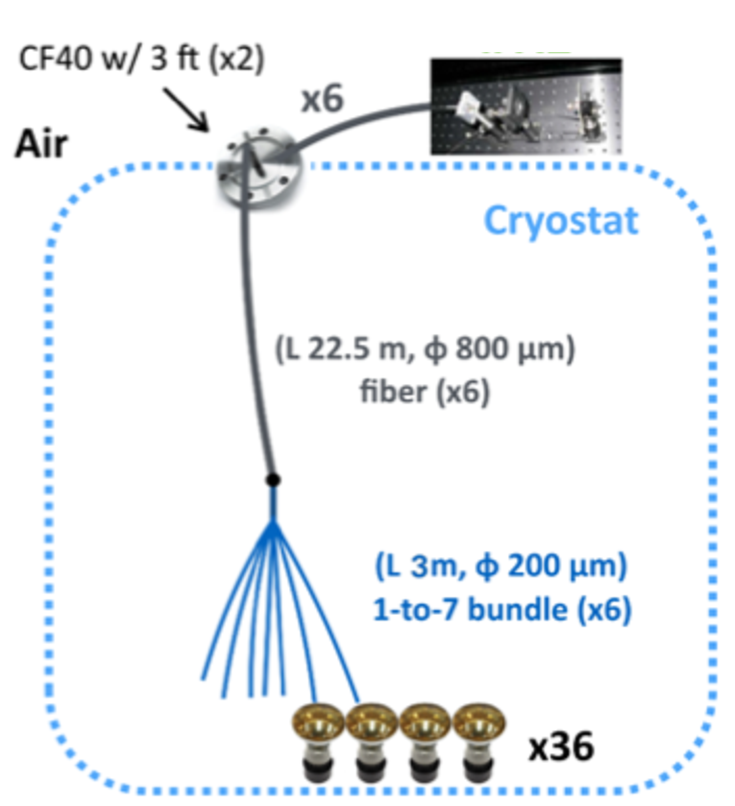
\includegraphics[width=0.4\textwidth]{dppd_5_1}
\end{dunefigure}

Assuming the ProtoDUNE-DP design for the DUNE FD with 720 PMTs, 120 bundles, 120 fibers, 120 light sources, 120 flange feedthroughs, and 20 reference sensors will be needed. The length of the fibers and bundles has to be calculated considering the exact position of the feedthrough flanges. The number of flanges required to host 120 SMA feedthroughs will depend on their size. However, alternatives to this design will be pursued with R\&D measurements in order to reduce the amount of fibers and increase the input light if necessary. In order to reduce the number of fibers, light diffusers can be used, so that one fiber can illuminate at least 4 PMTs. For instance, a diffuser could be placed at the ground grid. 

%%%%%%%%%%%%%%%%%%%%%%%%%%%%%%%%%
\subsection{Validation Tests}
\label{sec:fddp-pd-5.2}

In order to validate the design, the most important result will come from the ProtoDUNE-DP performance. In any case, since the fibers to be used in DUNE DP will be longer, dedicated calculations and measurements to confirm that sufficient light reaches the PMTs will be performed. Also, alternative designs, will be validated in different laboratories. Using a diffuser placed in the ground grid can be tested in a vessel. The light source will also be validated by studying the different options in the lab. All these measurements will be performed at room temperature and in liquid nitrogen to test the behavior at cryogenic temperatures.

Once the design is fixed, basic characterization measurements will be performed on the fibers upon receiving them from the manufacturer. Those measurements will consist of providing light with a known source and measuring the output with a power meter. Measurements at cryogenic temperatures may not be needed at this point.

Finally, during the photon calibration system installation, each fiber and source will be re-tested to check that the expected light is arriving to each PMT using a photodiode. A dedicated procedure will be designed with this purpose, similar to the one used in ProtoDUNE-DP.

%%%%%%%%%%%%%%%%%%%%%%%%%%%%%%%%%%%%%%%%%%%%%%%%%%%%%%%%%%%%%%%%%%%%
\section{Photon Detector Performance}
\label{sec:fddp-pd-6}

To define the PDS performance a good understanding of the light generation is needed. For this, optical simulations and a good knowledge of the light properties is required. The DUNE experiment expects to record not only accelerator neutrino interactions, but also rare non-beam events such as supernova neutrino bursts or nucleon decays. In those cases, an internal trigger is required: an optimized light collection system is hence mandatory. This section will describe the tools developed in the consortium for the light simulation in large detector volumes for these purposes.

The main feature of a LAr TPC detector is to collect electrons produced by the energy loss of charged tracks when crossing the volume. This signal provides a high resolution 3D image of the event. The reconstructed topology and the amount of charge collected gives the characterization of the tracks (identification and energy). Together with the charge, scintillation light is also produced in LAr. There are many advantages to collect and study the scintillation signal. As only a fraction of the initial energy deposition is converted into electrons, the rest being emitted as photons, light collection can improve the calorimetry of the detector. A fast (few ns) and a slow (few $\mu$s) time constants drive the emission of the light. The light signal can provide the $t_0$ of the event, which is a necessary observable for a proper reconstruction. The study of the slow component can give insights into the purity of the LAr. 

When energy deposition occurs, either the knocked argon atom gets excited or an electron is ejected. For the latter case, the electron has a probability to be recaptured by an argon ion, which depends on the drift field and on the amount of energy deposited. In this case, an excited argon state is also produced. In order to decay to ground state, the excited argon will combine with another argon atom, to form an excited eximer. A photon at 128\,nm will then be emitted to allow the eximer to return to ground state. As the eximer can be formed in a singlet or triplet state, two time constants will be observed: the singlet at 6\,ns and the triplet at 1.6\,$\mu$s. These principles are sketched in Fig. \ref{fig:dppd_6_0}.

\begin{dunefigure}[A sketch depicting the mechanism of light production in argon.]{fig:dppd_6_0}
{A sketch depicting the mechanism of light production in argon.}
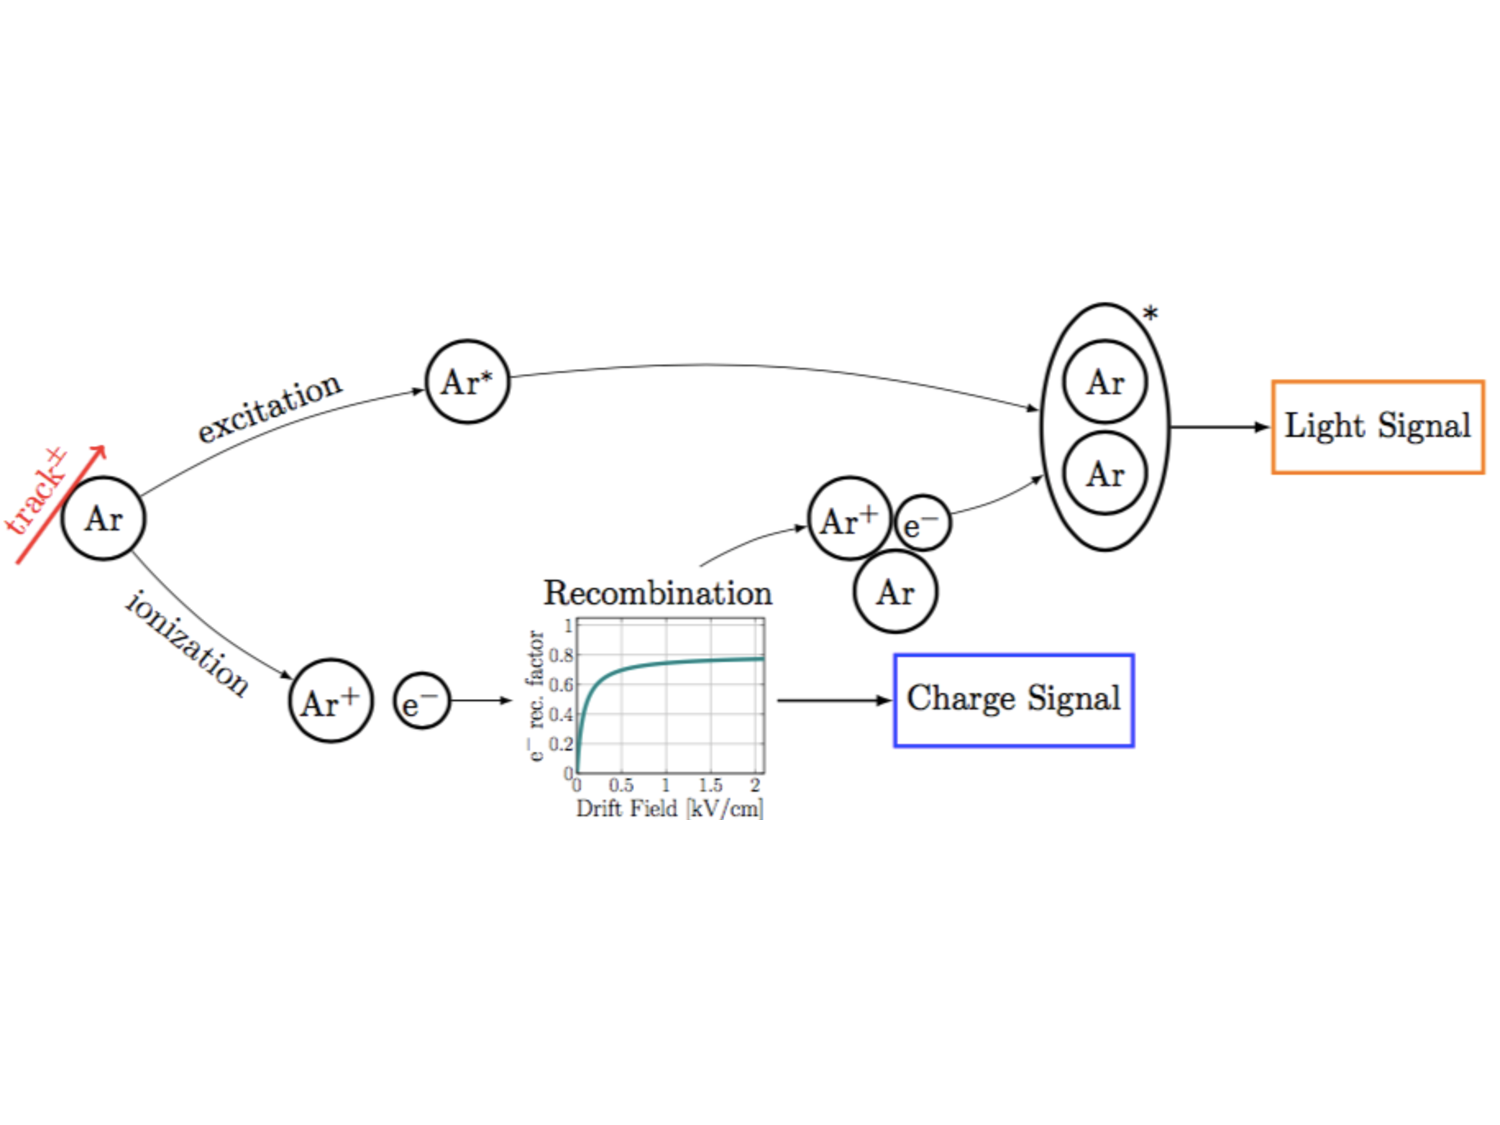
\includegraphics[width=0.8\textwidth]{dppd_6_0}
\end{dunefigure}

% \begin{dunefigure}[A sketch depicting the mechanism of light production in argon.]{fig:dppd_6_0}
% {A sketch depicting the mechanism of light production in argon.}
% \begin{tikzpicture}
% \node[circle, very thick,draw=black, fill=white, inner sep=0pt,minimum size=.9cm, text=black] (ini) at (0,0) {Ar};
% \draw[very thick,red,->](-.95, -.5) -- (0,.8) node [pos=.5, color=red, above, sloped] {track$^\pm$};
% \node[circle, very thick,draw=black, fill=white, inner sep=0pt,minimum size=.9cm, text=black] (exc) at (4,1.5) {Ar$^*$};
% \draw[-latex, bend left=10] (ini) to node[pos=.5, sloped, above] {excitation} (exc);
% \node[circle, very thick,draw=black, fill=white, inner sep=0pt,minimum size=.9cm, text=black] (ion) at (2.5,-2) {Ar$^+$};
% \node[circle, very thick,draw=black, fill=white, inner sep=0pt,minimum size=.6cm, text=black] (ele) at (3.5,-2) {e$^-$};
% \draw[-latex, bend right=10] (ini) to node[pos=.5, sloped, below] {ionization} (ion);
% \draw[-latex] (ele) to (4.5, -2);
% \begin{scope}[xshift=5.2cm, yshift=-2.8cm, scale=0.3]
% \begin{axis}[
% 		axis line style = thick,
%         domain=0.001:2.1,
%         xmin=0., xmax=2.1,
%         ymin=0, ymax=1.05,
%         samples=400,
%         grid=major,
%         xlabel={Drift Field [kV/cm]},
%         ylabel={e$^-$ rec. factor},
%         label style={font=\Huge},
%         tick label style={font=\huge} 
%         ]
%         \addplot+[mark=none, line width=4pt, teal] {0.8/(1+0.0741/x)};
%  \end{axis}
%  \end{scope}
% \node (rec) at (6.1, -0.8) {Recombination};
% \node[circle, very thick,draw=black, fill=white, inner sep=0pt,minimum size=.9cm, text=black] (ion2) at (8.2,0) {Ar$^+$};
% \node[circle, very thick,draw=black, fill=white, inner sep=0pt,minimum size=.6cm, text=black] (ele2) at (9,-0.05) {e$^-$};
% \node[circle, very thick,draw=black, fill=white, inner sep=0pt,minimum size=.9cm, text=black] (ato) at (8.7,-0.8) {Ar};
% \draw[-latex, bend left = 10] (rec) to (ion2);
% \node[ellipse, very thick, draw=black, fill=white, minimum height=2.7cm, minimum width=1.4cm] (ell) at (11,1) {};
% \node[text=black] at (11.5, 2.2) {*};
% \node[circle, very thick,draw=black, fill=white, inner sep=0pt,minimum size=.9cm, text=black] (exc1) at (11,1.5) {Ar};
% \node[circle, very thick,draw=black, fill=white, inner sep=0pt,minimum size=.9cm, text=black] (exc2) at (11,0.5) {Ar};
% \draw[-latex, bend left = 10] (exc) to (ell);
% \draw[-latex, bend right = 10] (ele2) to (ell);
% \node (light) at (14, 1) [draw=orange,very thick,fill=white, minimum width=2cm,minimum height=1cm] {Light Signal};
% \draw[-latex, thick](ell) to (light);
% \node (charge) at (10, -2) [draw=blue,very thick,fill=white, minimum width=2cm,minimum height=1cm] {Charge Signal};
% \draw[-latex, thick](7.4, -2) to (charge);
% \end{tikzpicture}
% \end{dunefigure}

In the DP technology, due to the amplification area, there are two light signals produced. The first one, S1, is made by scintillation processes when a charged particle crosses the LAr volume. The second signal, S2, is produced in the gaseous phase. As the drifting electrons enter in high field regions (such as the extraction field or the amplification field in the LEMs), their velocities increase and Townsend avalanches occur. The current of electrons will produce electroluminescence light with the same wavelength and similar time structure as for the S1 signal. The minimum field needed to produce electroluminescence is $\sim$3.5\,kV/cm at the gas density at cryogenic temperatures. The S2 light is expected to be an irreducible background for the light studies in ProtoDUNE-DP, as the detector will be on the surface. Indeed, the S2 signal can last as long as the total drift time of the electrons: 0.625\,ms per meter of drift at a drift field of 500\,V/cm.

The LAr optical properties are the subject of significant discussions in the community, in particular regarding the LAr absorption length and the Rayleigh scattering length. The former will affect the light yield collected whereas the latter will impact mostly its uniformity. 

Table~\ref{tab:dppd_t_6_0} summarizes the default optical parameters chosen for the light simulation methods described in the following subsection. The absorption/reflection of the VUV photons on stainless-steel (constituting the drift cage, cathode, extraction grid and ground grid) and on copper (on the LEM surfaces) are poorly known. The knowledge of those reflection coefficients is limited by the fact that they depend strongly on the polishing procedure. Hence, one cannot rely on the literature as the tooling will certainly be different. The electroluminescence gain G, defined as the number of S2 photons produced per extracted drifting electron, is also subject to discussion. Experimental measurements of G have been performed in a setup quite similar to the amplification design of the DP technology, although the amount of photons emitted were measured above the LEM. In our case, the S2 photons are the ones leaving the LEM from below, which can be significantly lower. The measurement of the quantum efficiency of the PMTs at vacuum ultra-violet (VUV) wavelengths requires a specific setup operating in vacuum as VUV photons are absorbed in air. For the construction of the DP demonstrator, the PMT quantum efficiencies were measured before and after the TPB coating (a wavelength shifter used to convert 128\,nm photons to 435\,nm) using a LED that could emit light in the [200, 800]\,nm range.

\begin{dunetable}
[Default optical properties. Below the thick line are presented some quantities used in our studies although they are not linked to the optical properties of the LAr.]
{lcc p{0.8\textwidth}}
{tab:dppd_t_6_0}
{Default optical properties. Below the thick line are presented some quantities used in our studies although they are not linked to the optical properties of the LAr.}
 & VUV photons & Shifted photons \\ 
 & $\lambda = 128$\,nm & $\lambda = 435$\,nm\\ \toprowrule
 Absorption length & \multicolumn{2}{c}{$\infty$} \\ \colhline
 Rayleigh scattering length & 55\,cm & 350\,cm\\ \colhline
 Absorption coefficients & 100\% & 50\% \\ \colhline
 LAr refractive index & 1.38 & 1.25\\ \colhline
 PMT quantum efficiency & \multicolumn{2}{c}{0.2 }\\ \colhline
 Electroluminescence gain & 300\\ \colhline
\end{dunetable}

To understand the performance of the PDS, we need to take into account the following indicators:
\begin{itemize}
\item Overall detected light yield, in PEs per MeV of deposited energy in LAr
\item Uniformity of the light yield across the entire LAr TPC active volume
\item Event time resolution extracted from the detected photon signal 
\end{itemize}

In turn, these indicators will directly impact the strategy and performance of the DUNE trigger system (Sec.~\ref{sec:fddp-pd-7}), and will determine whether the photon detector technical design is sufficient to meet the DUNE physics goals. These higher-level studies will be available on the TDR timescale.  Our current understanding of the performance indicators listed above is largely based on ProtoDUNE-DP simulations. The current status of the simulation work is discussed in detail in Sec.~\ref{sec:fddp-pd-6.1}, work is focused on ProtoDUNE-DP in a first phase, and then will be expanded to DUNE DP FD. For a realistic ProtoDUNE-DP geometry, an average light yield of 6 PEs/MeV is expected across the entire active volume. This promising yield is obtained  by assuming thirty-six 8-inch PMTs located below the ProtoDUNE-DP cathode plane, averaging to one PMT per m$^2$. On the other hand, spatial non-uniformities in the photon detector response are found to be important and need to be modeled in detail. Variations as large as one order of magnitude both parallel to the drift direction (due to geometrical effects and absorption of light by LAr) as well as perpendicular to it (due to light absorption on detector boundaries) are obtained. The event time resolution due to light production and light propagation times, hence neglecting electronics and DAQ effects for now, is expected to be of order $\mathcal{O}$(100\,ns) and hence largely sufficient for our purposes. These initial low-level performance estimates will be refined with more realistic simulations and with ProtoDUNE-DP data (Sec.~\ref{sec:fddp-pd-6.2}) in the future. They will also be extended to the full FD geometry on the TDR timescale.

%%%%%%%%%%%%%%%%%%%%%%%%%%%%%%%%%
\subsection{Simulations}
\label{sec:fddp-pd-6.1}

At zero drift field, when the electron recombination is maximum, roughly 40$\times10^3\,\gamma$/MeV are produced. At the nominal drift field of 500\,V/cm, then 24$\times10^3\,\gamma$/MeV are generated. For reference, the energy deposited by a mip track is 2.12\,MeV/cm. Given the size of the ProtoDUNE-DP ($6\times6\times6$\,m$^3$) and the fact that it is located on surface, roughly 100 muons are expected to cross the fiducial volume during the 4\,ms time window of the data acquisition. With a full Geant4 \cite{geant4} simulation, it takes roughly 3 h 30 to propagate all the photons emitted by a single MIP track crossing the ProtoDUNE-DP detector. A full optical simulation is hence computationally prohibitive. Three simulation approaches are being explored to provide a light simulation needed for the design optimization of the DUNE FD module described in the following.


\subsubsection{Generation of light maps}
\label{subsec:fddp-pd-6.1.1}

In this method, the photons are propagated in a full dedicated Geant4 simulation only once. The main light characteristics (photon detection probability called visibility hereafter, and time profile) needed for light studies are stored in a map in a ROOT \cite{root} file format which can be then read by any other simulation program. This work was done first using LightSim, a dedicated software developed at LAPP. These maps have been adapted to be read by LArSoft and work is on-going to directly generate them in LArSoft where light maps are known as photon libraries. In particular S2 light needs to be simulated in LArSoft for the first time, as no previous efforts on DP technology were done.

In the dedicated Geant4 code, special care has been taken to precisely describe all sub-detector components that might affect the light propagation: LEM plates, extraction grid, field cage rings, the cathode and its supporting structure and the ground grid above the PMTs. The LAr fiducial volume is then divided into voxels of 25\,cm$^3$ and $10^7$ photons are isotropically generated at the center of each voxel. The number of photons reaching each PMT, and their arrival times are stored. The light map can then be built from these results. For each voxel and for each PMT, the visibility is computed as: $w=N\gamma^{\textrm{collected}}/N\gamma^{\textrm{generated}}$. In order to be able to reproduce the time profile, each distribution is fit to a Landau function. From the fits, three parameters are extracted: the minimum time for photons to arrive to the PMT, $t_0$; the peak of the distribution, $t_{\textrm{peak}}$ from the Landau most probable value (MPV); and the distribution spread, the $\sigma$ of the Landau function. These three parameters are stored in the light maps together with the photon detector identifier. The same procedure is done for the gaseous phase, although the 
voxel size is smaller in height (only 5\,mm) and the number of photons generated is higher in order to get sufficient statistics. In Fig.~\ref{fig:dppd_6_1_1_ab}, two fitted time distributions are presented. As one can see, the shapes of the time distributions depend strongly on the source to PMT distance. For close sources, the distributions are very sharp and the Landau description may not be the optimal function to use. On the other hand, when the distance is wider, the distribution is broader and the Landau fit reproduces quite well the simulations. In order to minimize the amount of parameters to be stored in the map, the Landau descriptions for all cases were kept as only a small fraction of the fits could be considered problematic.

\begin{dunefigure}[Landau fits (red line) of the travel time distributions (black histogram) for a source close (left) and far (right) to the PMT.]{fig:dppd_6_1_1_ab}
{Landau fits (red line) of the travel time distributions (black histogram) for a source close (left) and far (right) to the PMT.}
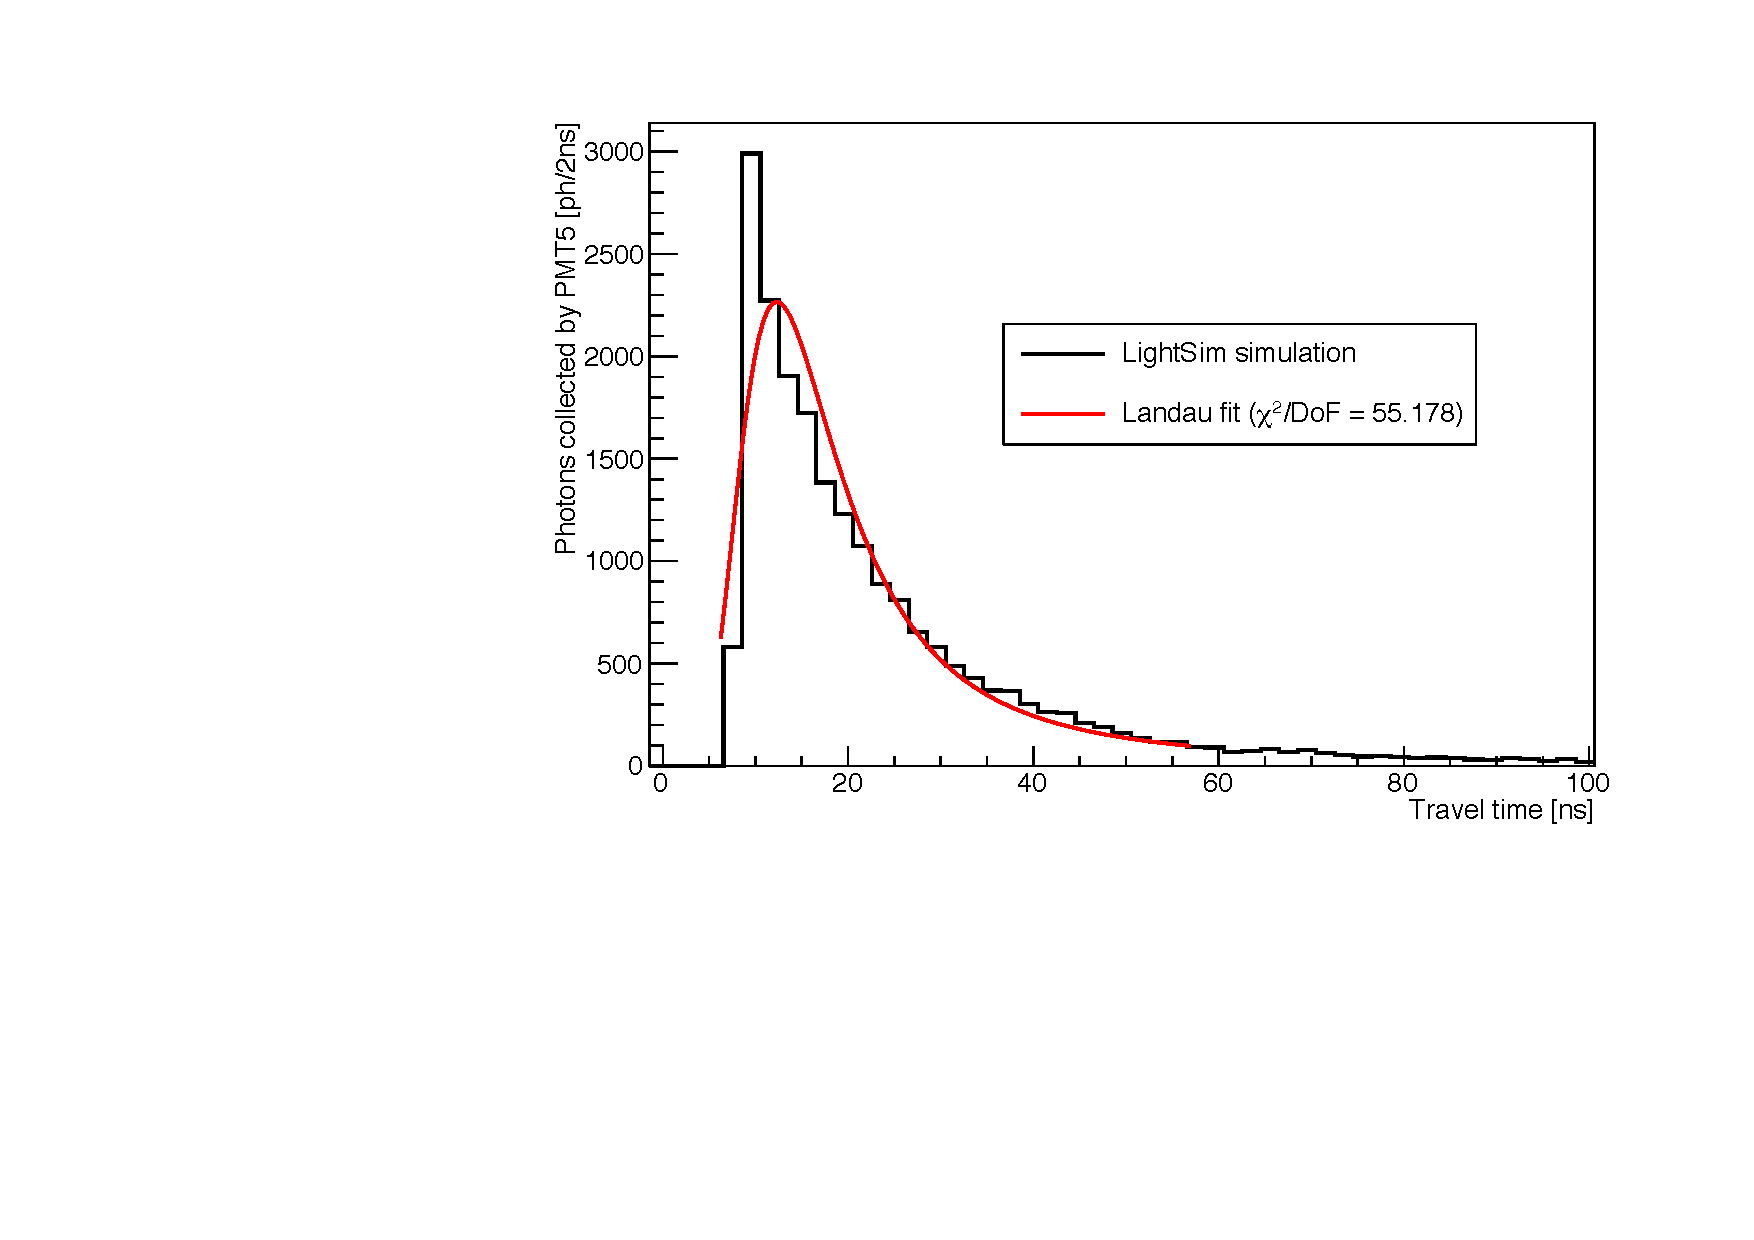
\includegraphics[width=0.45\textwidth]{dppd_6_1_1_a}
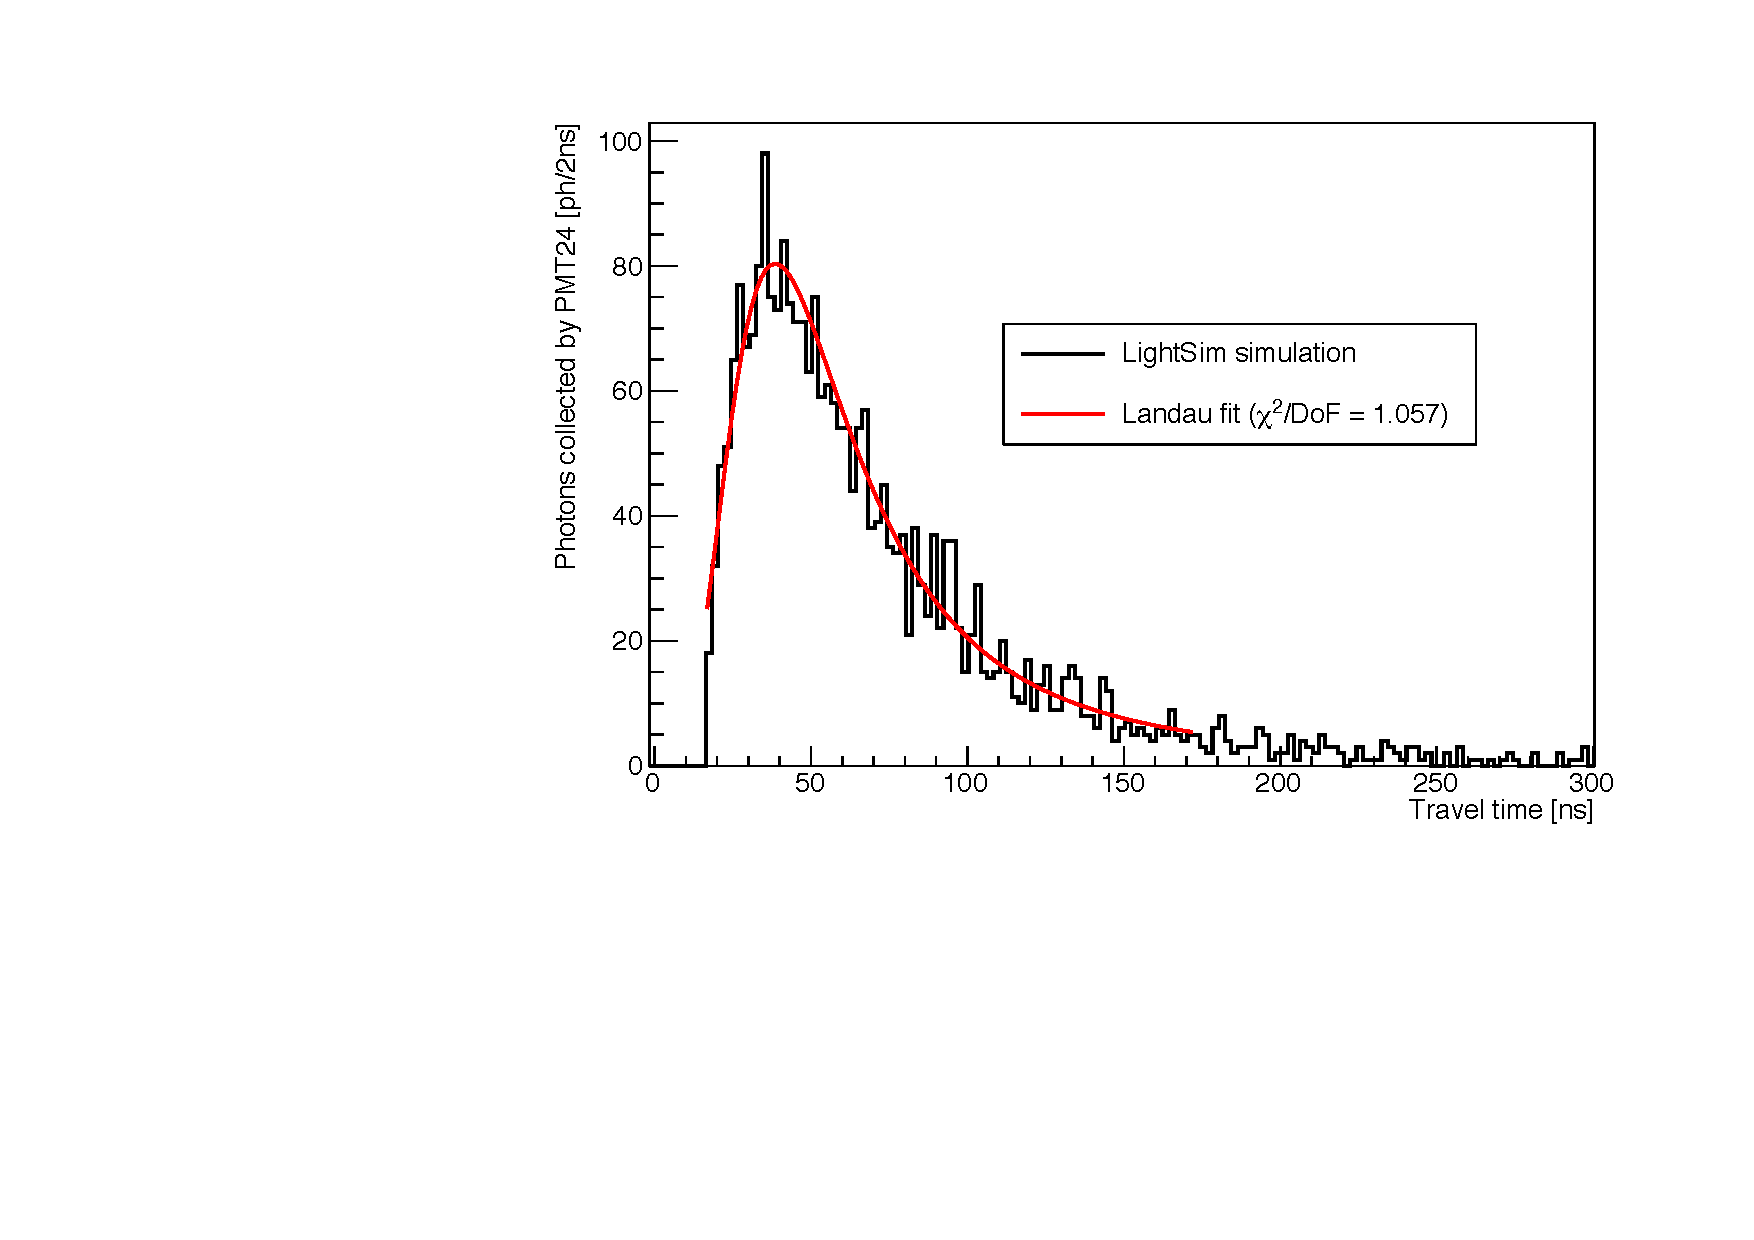
\includegraphics[width=0.45\textwidth]{dppd_6_1_1_b}
\end{dunefigure}

The light collected per PMT can be simulated together with the charge for crossing tracks in a standard simulation code where a detailed description of the detector is not needed. At each step of the track propagation, the energy deposited is computed by Geant4. This energy is converted into number of electrons and photons produced. The drift of the electrons to the readout is not simulated, and effects due to the absorption by impurities, electron cloud diffusion or non-uniform drift electric field are parametrized. As for the light simulation, the number of photons reaching each PMT and their time of arrival are obtained from the light maps. As the map has been computed with discrete entries, an interpolation of the four light parameters ($w$, $t_0$, $t_{\textrm{peak}}$, $\sigma$) between the actual source position and the closest voxel centers is performed. An example of the evolution of the visibility and its 3D interpolation is presented in Fig.~\ref{fig:dppd_6_1_1_cd}. The loss of photons due to the cathode and ground grid are visible. Given the ProtoDUNE-DP cathode and supporting structure design, and considering the default optical parameters presented in Table~\ref{tab:dppd_t_6_0}, it has been shown that up to $\sim$70\,\% of the photons generated in the active volume are absorbed by those structures before reaching the PMT array.

During the generation of the light maps, the light propagation parameters are the ones presented in Table~\ref{tab:dppd_t_6_0}. One can study afterwards the loss of photons due the LAr absorption length using an approximation of the probability of the photon to be absorbed by the medium as: $p_{\textrm{abs}} = \exp(-\frac{D_{\textrm{travel}}}{\lambda_{\textrm{abs}}})$. For the study of other light propagation parameters (Rayleigh scattering length and absorption on the stainless-steel and copper) new maps have to be generated.

The light maps generation is a long process. It takes roughly 3 days of computing time to generate the maps for ProtoDUNE-DP, even though only 1/8$^{th}$ of the voxels were simulated as the detector and the PMT positionig is symmetric. Generating maps for larger volumes such as the DUNE FD module, where the maximum source to PMT distance will be around 60\,m, could be too much time consuming. Moreover, the light simulation in the FD is foreseen to drive the optimization of the positioning of the PMTs and will guide the studies of possible implementation of light reflectors. As most of the light propagation parameters in LAr are still subject to large uncertainties, these studies will have to be performed considering various absorption and diffusion values. Therefore, it is crucial to be able to have a faster way to get a quite reliable light simulation, at the cost of losing some precision.

\begin{dunefigure}[Evolution of the visibility seen by a central PMT (pointed by the arrow) as a function of different source positions in $x$ and $z$ ($y$ is set at 0\,mm). The position of the cathode and the ground grid are highlighted.]{fig:dppd_6_1_1_cd}
{Evolution of the visibility seen by a central PMT (pointed by the arrow) as a function of different source positions in $x$ and $z$ ($y$ is set at 0\,mm). The position of the cathode and the ground grid are highlighted. Left: discrete values from the maps, right: after 3D interpolation.}
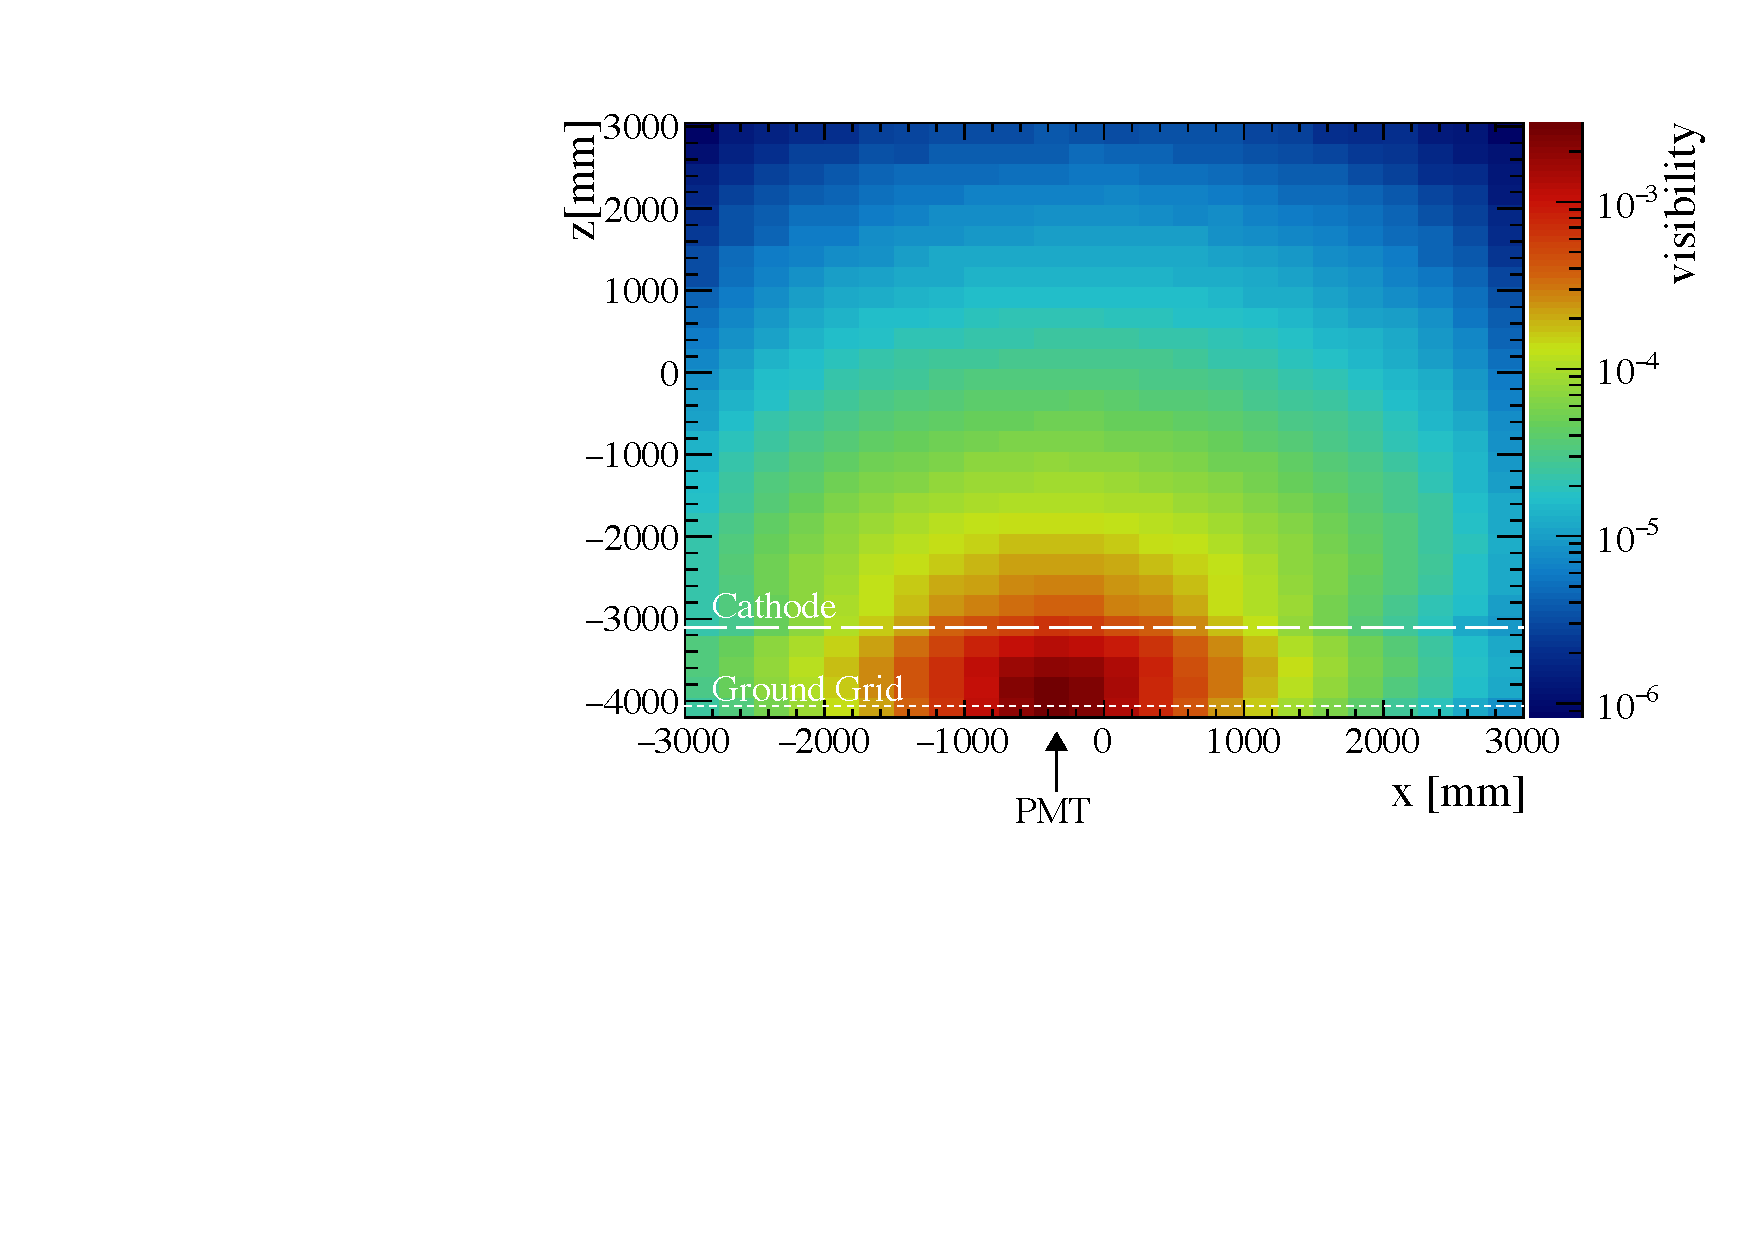
\includegraphics[width=0.45\textwidth]{dppd_6_1_1_c}
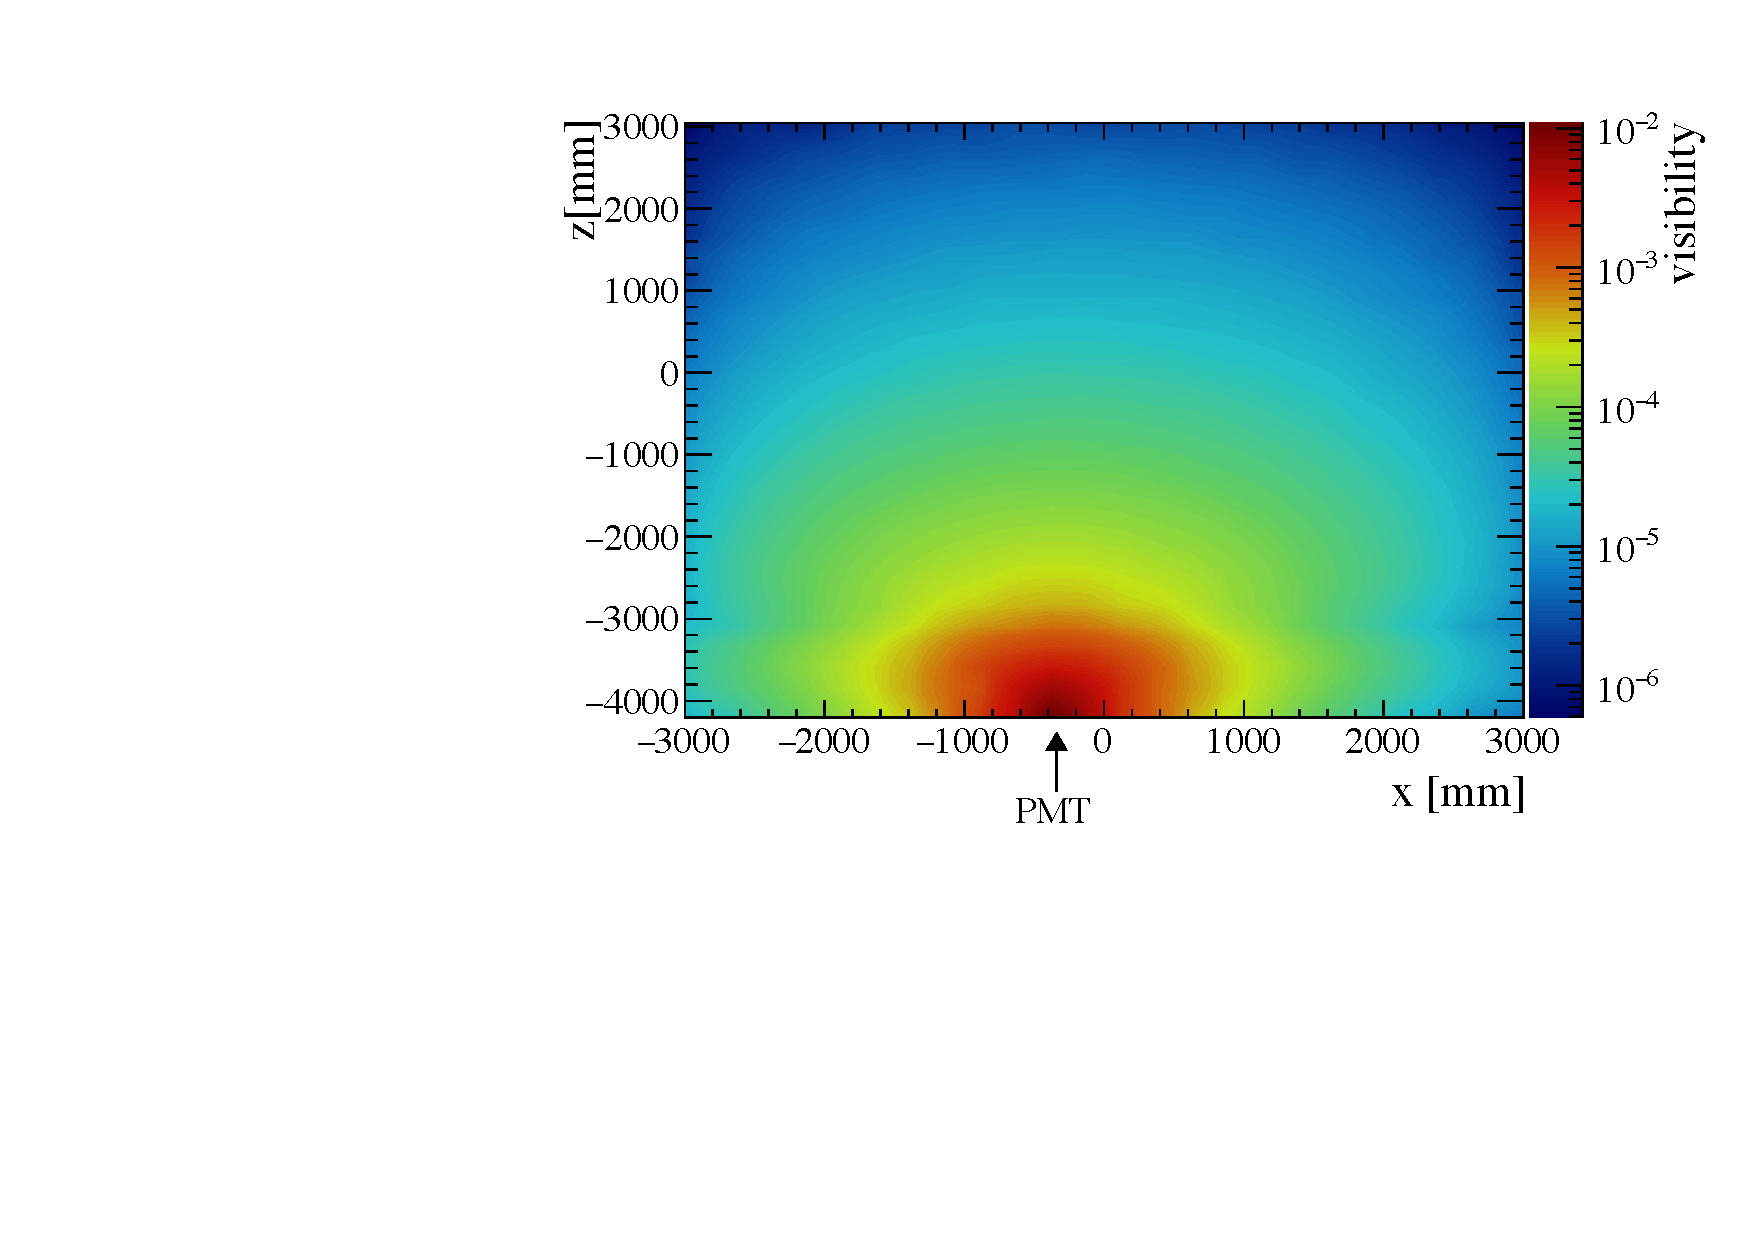
\includegraphics[width=0.45\textwidth]{dppd_6_1_1_d}
\end{dunefigure}

\subsubsection{Parametrization from the light maps}
\label{subsec:fddp-pd-6.1.2}

Without considering the border effects, where the photons are mostly absorbed, it is intuitive that the visibility and the time profile depend only on the source to PMT distance.

This approach has been followed for the SBND \cite{sbnd} light simulation and is considered for the DUNE-DP module as well. In Fig.~\ref{fig:dppd_6_1_2}, the evolution of the visibility and the peak time as a function of the source to PMT distance are shown. As these plots have been generated from the light maps, where the borders are taken into account,  the same evolutions are also presented only for voxels at least 1\,m away from the active volume boundaries. For the visibility, the structure is quite complicated when taking all the voxels highlighting the complexity of the light simulation in a closed space. When looking at voxels away from the boundaries, one can see a clear correlation between distance and visibility. As for the time distribution (here for the peak time, but same goes for $t_0$ and $\sigma$ parameters), one can notice two different regimes for short and large distance (the transition being at around 2\,m).

This preliminary study is quite encouraging for the light simulation in the FD module, at least for light sources being far away from the fiducial volume boundaries. As it is complicated to disentangle the effects due to the propagation and absorption parameters from the light maps, a carefull dedicated study should be performed in order to get parametrization of the visibility and time distribution parameters as a function of the photon travelling distance.

\begin{dunefigure}[Evolution of the visibility and peak time as a function of the source-PMT distance as simulated in the ProtoDUNE-DP geometry (Preliminary study).]{fig:dppd_6_1_2}
{Evolution of the visibility (top) and peak time (bottom) as a function of the source-PMT distance as simulated in the ProtoDUNE-DP geometry (Preliminary study). On the left, all voxels are considered, on the right only the voxels at least 1\,m away from the fiducial border are considered.}
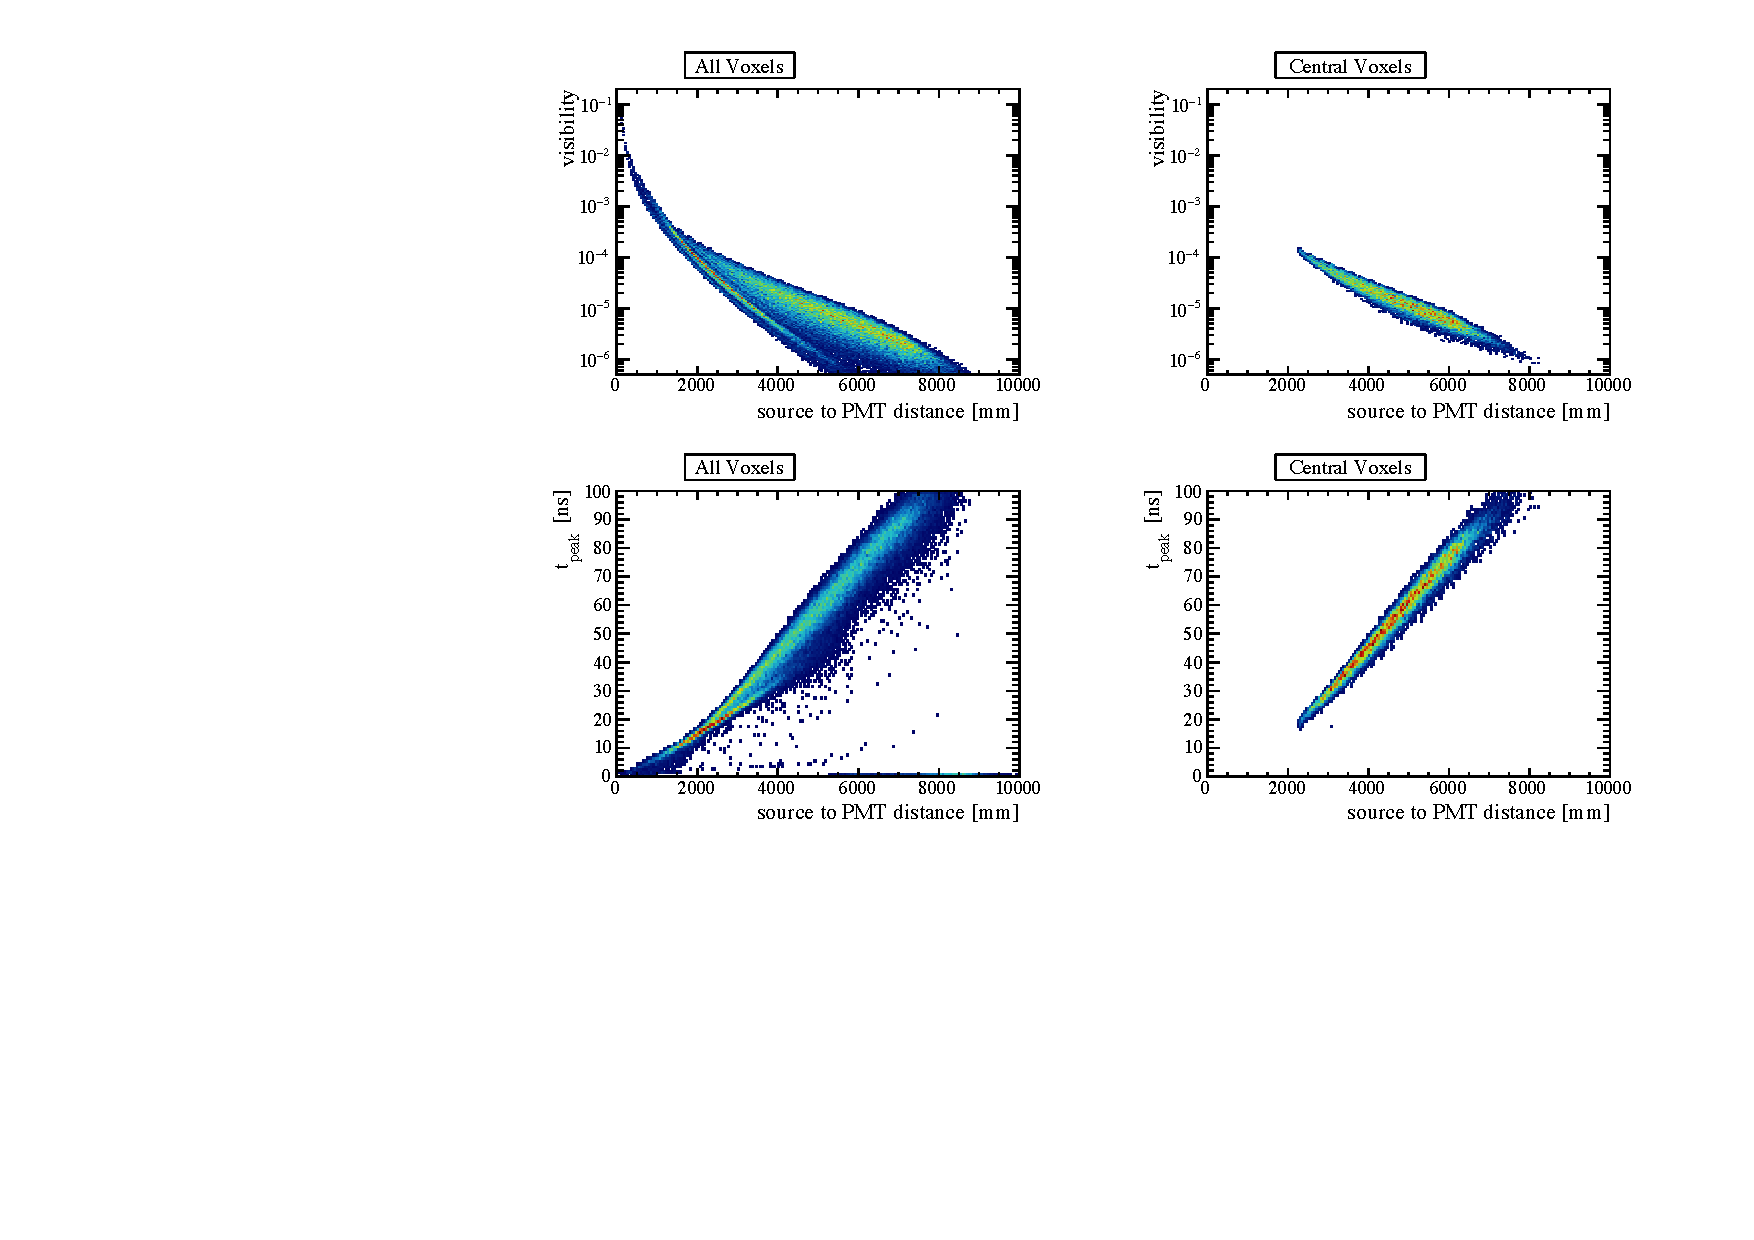
\includegraphics[width=0.8\textwidth]{dppd_6_1_2}
\end{dunefigure}

\subsubsection{Analytical approach}
\label{subsec:fddp-pd-6.1.3}

The propagation of light in a uniform material such as LAr can be described by the Fokker-Planck diffusion equation:

$$\frac{\partial}{\partial t}p(x,y,z,t) = D\left[\frac{\partial^2}{\partial x^2}p(x,y,z,t) + \frac{\partial^2}{\partial y^2}p(x,y,z,t) + \frac{\partial^2}{\partial z^2}p(x,y,z,t)\right]$$ 

where $D$ is the diffusion coefficient. In an unbound medium, the Fokker-Planck equation is solved by the Green function:

\begin{eqnarray*}
G(\textbf{r}, t; \textbf{r}_0, t_0) &=& \frac{1}{[4\pi D c (t-t_0)^{3/2}]}\exp\left(-\frac{|\textbf{r}-\textbf{r}_0|^2}{4Dc(t-t0)}\right) \\
D &=& \frac{1}{3(\mu_A + (1-g)\mu_S)}
\end{eqnarray*}

where $\mu_A$ and $\mu_S$ are the absorption and scattering coefficients respectively (both in units of m$^{-1}$), $g$ is the average scattering cosine ($g = 0.025$). In LAr with the default optical properties of Table \ref{tab:dppd_t_6_0}, $D = 18.8$\,cm. In a bound medium, with full absorption of the photons by the field cage and LEMs, a few additional techniques have to be used to obtain a solution. With this method, it takes only a few ms to have the photon density at a given photon detector from a specific point source. From preliminary studies, a relatively good agreement between analytical approach and full simulation has been found. In particular, the arrival time distributions of photons on the PMTs are well reproduced. The only drawback is that one cannot easily implement/study a complicated geometry including regions that are semi-transparent to light. Hence, the comparisons of the visibilities that one gets from the two methods are not in agreement in the overall light yield, but have a very similar trend in terms of spatial dependences. Some studies are ongoing in order to improve the analytical method results as this approach could be extremely powerful for physics studies in the FD module.

%%%%%%%%%%%%%%%%%%%%%%%%%%%%%%%%%
% \subsection{Event Reconstruction}
% \label{sec:fddp-pd-6.2}

\subsection{Use of light data in DP prototypes}
\label{sec:fddp-pd-6.2}

The DP demonstrator (WA105 $3\times1\times1$\,m$^3$) was operated from June to November 2017 with cosmic data. About 5 million light events were taken with various high voltage configurations. The study of the S1 light as a function of the drift field was performed. An example of an averaged waveform fitted to a fast and a slow scintillation components is shown in Figure \ref{fig:dppd_6_2}. The amount of S2 light can be monitored as a function of the extraction and LEM amplification fields.

\begin{dunefigure}[]{fig:dppd_6_2}
{Averaged waveform of the S1 light signal taken with one PMT from the WA105 $3\times1\times1$\,m$^3$ LAr DP TPC, fitted with a function (red line) that is the sum of a Gaussian, parametrized by t$_0$ and $\sigma$, and two exponential functions, with decay time constants $\tau_{fast}$ and $\tau_{slow}$, and normalization factors $A_{fast}$ and $A_{slow}$}
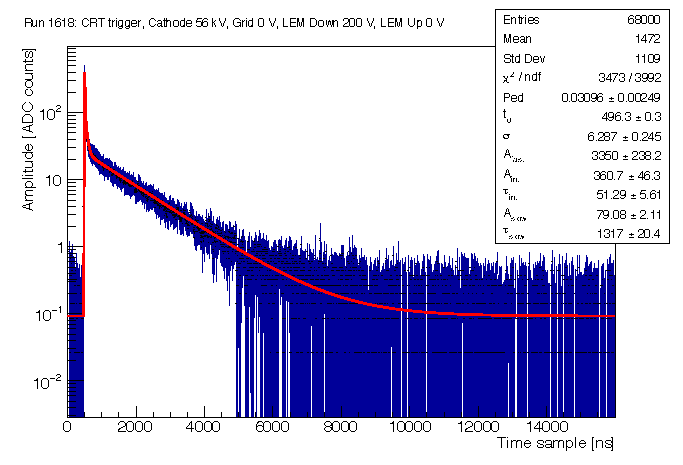
\includegraphics[width=0.6\textwidth]{dppd_6_2}
\end{dunefigure}

Light maps have also been generated with the demonstrator geometry, and data/MC comparisons are ongoing. The preliminary results look promising, although the statistics in each settings and the relatively small size of the detector still constitute a challenge to extract the entire optical properties of the LAr.

%%%%%%%%%%%%%%%%%%%%%%%%%%%%%%%%%%%%%%%%%%%%%%%%%%%%%%%%%%%%%%%%%%%%
\section{Photon Detector Operations}
\label{sec:fddp-pd-7}

%%%%%%%%%%%%%%%%%%%%%%%%%%%%%%%%%
%\subsection{Data Path and Event Format}
%\label{sec:fddp-pd-7.1}

%%%%%%%%%%%%%%%%%%%%%%%%%%%%%%%%%
\subsection{Trigger Strategy}
\label{sec:fddp-pd-7.2}

As explained in section \ref{sec:fddp-pd-1.5}, the PDS can operate in different acquisition modes depending on the trigger. These modes include the external trigger, which is the case of the beam events; the trigger for non-beam events such as SN bursts; the continuous mode; and the calibration mode. 

In the LAr TPC there are different uses of the light signal: cosmic ray/track timing for the reconstruction; non-beam events trigger such as SN neutrino burst, atmospheric neutrinos, and proton decay; and calorimetry, as the light and charge signal are anti-correlated. These physics studies imply different requirements in terms of dynamics of the electronics and data sampling. For example, the light from a 50\,kpc supernova explosion will be at the PE level, a proton decay signal will be at a few hundreds (integrated) PE level and most of the light signal from neutrino interactions used for the calorimetry will be at much higher level. 

As far as the non-beam events trigger strategies are concerned, again the requirements can be very different. In the event of a nearby (10\,kpc) SN burst, it is expected that a few thousands of neutrinos will homogeneously interact in the detector for a period as long as $\sim$10\,s. Hence, the SN burst trigger strategy is mostly driven by the energy threshold set for $\nu$ detection and its efficiency: 30\,MeV is sufficient for a galactic SN, 5\,MeV is needed for a burst in Andromeda. %As if such explosion occurs during data taking, the normal detector DAQ will be stopped to collect as much SN $\nu$ events as possible, one can also design a combined charge and light trigger in order to minimize the amount of false triggering.

%The detection of a proton-decay-like event in a large LAr volume is a much more complicated task. 
A high-efficiency trigger for single proton decay events has to be designed considering the worst case scenario, e.g. the event happening at the top of the detector, 12\,m away from the closest PMT. On top of it, if an $^{39}$Ar decay occurs close to a PMT, the light collected will be very similar to the one expected from proton-decay signal. Hence, in order to minimize the amount of false triggers, one can think of PMT thresholds for a cluster of close-by PMTs.

All these important studies will be further investigated once a reliable light simulation of the DP far detector module will be available. For the DP technology, the main light trigger concerns are the amount of light collectable for a photon traveling distance of 12\,m and the S1/S2 separation. Luckily, the data that will be collected in the ProtoDUNE-DP in 2018 will provide crucial inputs for the optimization of the DP far detector light collection system and for the design of an efficient trigger strategy for rare non-beam events. 

%%%%%%%%%%%%%%%%%%%%%%%%%%%%%%%%%
\subsection{Data Quality Monitoring}
\label{sec:fddp-pd-7.3}

The PMTs installed at the bottom of the tank will be operated for 10-20 years with no possibility to access them. Monitoring tools to ensure data quality of the PDS will have to be developed to catch any malfunctioning detector before data analysis. For instance, the amount of dark noise and the stability of the PMT response will have to be monitored over time. For the gain evolution, either studies of standard candles, e.g. from Michel electrons or average collected light produced by cosmic tracks, or with the dedicated calibration system are considered.

Monitoring tasks were performed during the 6 months of operation of the WA105 $3\times1\times1$\,m$^3$ with no dedicated light calibration system. As the gain and noise calibrations were performed at room temperature before the PMT installation, similar measurements are foreseen in the next months in order to quantify the possible degradation of the photomultipliers and/or the TPB layer. This and the forthcoming operation of the ProtoDUNE-DP, will again provide crucial input towards the PDS monitoring system in the FD module.

%%%%%%%%%%%%%%%%%%%%%%%%%%%%%%%%%%%%%%%%%%%%%%%%%%%%%%%%%%%%%%%%%%%%
\section{Interfaces}
\label{sec:fddp-pd-8}

The PDS will have several interfaces with other subsystems and the global DUNE systems. The interface documents related to DP PDS are given in Table~\ref{tab:dppd_t_8}. Only part of the basic interfaces are summarized below. 

\begin{dunetable}
[DPPD interface documents]
{|l|c| p{0.8\textwidth}}
{tab:dppd_t_8}
{DPPD interface documents}

DPPD Interface Document & DUNE docdb number \\ \toprowrule
DP Electronics & 6772 \\
DP HV & 6799 \\
DAQ & 6802 \\
Cryogenic Instrumentation and Slow Control & 6781 \\
DUNE Physics & 7087 \\
Software and Computing & 7114 \\
Calibration & 7060 \\
Integration and Testing Facility & 7033 \\
Detector and Facilities (LBNF) Infrastructure & 6979 \\
Installation & 7006 \\
\end{dunetable}


\begin{itemize}

\item DP Electronics: The PDS will share the same front-end electronics standard as the charge readout, which is $\mu$TCA based \cite{utca}. Specifications of both PDS and front-end electronics will be determined by the simulations and ProtoDUNE-DP data.

\item HV: This interface includes the consideration of the distance between the cathode and the PMT planes, power dissipation from the PMTs and the combined impact on the simulations.

\item DAQ: The hardware interface will be mainly through optical fibers. DPPD will be providing data in continuous streaming and the interface will also include the DAQ software.

\item Cryogenic Instrumentation and Slow Control: The main interface points are the layout of the cryogenic instrumentation (e.g. purity monitors and light emitting system for the cameras) and the PMT support structures and cabling; and the slow control and the PDS power supplies and calibration system.

\item DUNE Physics: DPPD will have interfaces with the overall physics requirements on energy, time and angular resolution together with classification of events, decay modes and neutrino flavors.

\item Software and Computing: This interface will be on the development of simulation, reconstruction and analysis tools.

\item Calibration: The PSD will participate in the Global Calibration Task Force and will provide handles to allow global monitoring of the PMT performance.

\item Integration and Testing Facility: The operations at the Integration and Testing Facility are described in Section~\ref{sec:fddp-pd-9.2}. The interface items can be summarized as shipping and receiving of the DPPD components and basic testing and repairing at the facility. The interface also includes recycling/returning the packaging materials.

\item Detector and Facilities (LBNF) Infrastructure: DP PDS will have PMT support structures, cold cables routed in cable trays to the ceiling feedthrough flanges and racks and cable trays on top of the cryostat. Other interfaces with the facility include access to conventional facilities and participation in the detector safety systems. 

\item Installation: This interface will be through the transportation of the DPPD components to and between underground areas, clean room activities and storage, and installation coordination with the other teams. 

\end{itemize}

%%%%%%%%%%%%%%%%%%%%%%%%%%%%%%%%%%%%%%%%%%%%%%%%%%%%%%%%%%%%%%%%%%%%
\section{Installation, Integration and Commissioning}
\label{sec:fddp-pd-9}

%%%%%%%%%%%%%%%%%%%%%%%%%%%%%%%%%
\subsection{Transport/Handling}
\label{sec:fddp-pd-9.1}

The PMTs of the PDS will be shipped from various locations following the TPB coating and base electronics assembly. The shipping boxes will contain 24 PMTs resulting in 30 total deliveries of 720 PMTs. The PMTs will be individually wrapped with different wrapping materials for the coated window and the PMT base. The PMT-base wrappings will have special openings to enable the basic electronics tests at the Integration and Testing Facility.

The PMTs will be placed in modular shock absorbing assemblies inside the boxes. The assemblies will also allow a limited amount of safe inclination. The boxes will have integrated pellets for easy handling and short distance transportation. The PMTs will reach the Integration and Testing Facility by means of air and ground transportation. Each box will have a dedicated bar-code which will be visible on each side. This bar-code will also be associated with the shipping documents. 

%%%%%%%%%%%%%%%%%%%%%%%%%%%%%%%%%
\subsection{Integration and Testing Facility Operations}
\label{sec:fddp-pd-9.2}

The PMT boxes will be received by the Integration and Testing Facility (ITF). A shipping and delivery database will be managed by the ITF. The received status of the boxes will be available to the DPPD Consortium as the boxes arrive at the ITF. The PDS characteristics database managed by the DPPD Consortium will be updated accordingly to reflect the received status of the contents of the boxes. Each PMT assembly will have identifying bar-codes that will be directly connected to the PDS characteristics database. This database will store the PMT serial number, the base board serial number, special information about PTB coating and assembly if any, and performance and calibration characteristics. This database will form the basis of the operations database providing the initial calibration values and it will also store information about the ITF tests and underground installation and commissioning tests.

At the ITF, dedicated testing electronics will be connected to the PMTs through the special openings that allow access to the base boards. The test electronics will enable connecting several PMTs at a time. The tests will include basic functionality checks of both the PMTs and the base boards to assess the performance after transportation. No detailed performance characteristics will be measured at the ITF. The tests will be performed in a dedicated room with light and climate control. Once the performance of the PMTs in a box is validated, the boxes will be closed with the original covers. Before closing, additional quality checks on the shock absorbing assemblies will be made.

The preparation of the PMT boxes for underground transportation includes installing holding/lifting fixtures to the top and sides. The fixtures will allow crane operation. The boxes will be delivered to the surface station by ground transportation with relevant modification in the shipping database.

%%%%%%%%%%%%%%%%%%%%%%%%%%%%%%%%%
\subsection{Underground Installation and Integration}
\label{sec:fddp-pd-9.3}

Once the PMT boxes are underground, the same top and side covers will be opened as at the ITF. The PMTs will be carried to the underground storage area in sub-units of the shock absorbing assemblies which will be modular. The underground storage area for the PDS will be sufficiently large to store at least 30 PMTs for continuous installation operations.

The removal of the individual PMT wrappings will be done in the clean room. PMTs together with their base boards will go through visual inspection by the PDS installation supervisor. Once signed-off, the installation can proceed with multiple PMTs at a time by multiple teams. Cabling will be carried out in parallel and relevant database modifications will be made in-situ. The installation time management will be done in coordination with the cathode and field cage installation groups.

Following the mechanical mounting of the PMTs to the cryostat floor, the cables will be installed and routed through the cable trays. The bundles of cables will be routed through the cable trays along the cryostat walls from the PDS flanges. In parallel, the calibration fibers will be installed and routed through cable trays.

The underground operations will be performed under UV-blocked light.

%%%%%%%%%%%%%%%%%%%%%%%%%%%%%%%%%
\subsection{Commissioning}
\label{sec:fddp-pd-9.4}

The commissioning of the PDS will be performed in partitions. The size of the single partition will mainly be determined by the data acquisition system and the high voltage system. The data acquisition system and high voltage partitions will be commissioned, including the relevant control systems, prior to the connection of the PMTs to these systems. Once the physical sector corresponding to a partition is installed, the PMTs will be powered up and basic functionality and performance checks will be performed. These include pedestal data taking which consists of recording event data with external periodic triggering, and tests with the calibration system where the data taking is triggered in synchronization with a light source as described in Section \ref{sec:fddp-pd-5}.

As a result of the commissioning tests, the basic performance characteristics of the PMTs, e.g. the dark count rate and gain, will be measured in their final places. Installation-related issues will be identified and eliminated at this stage. A commissioned sector will be the part of the overall detector and can join the global calibration data taking and commissioning.

%%%%%%%%%%%%%%%%%%%%%%%%%%%%%%%%%%%%%%%%%%%%%%%%%%%%%%%%%%%%%%%%%%%%
\section{Quality Control}
\label{sec:fddp-pd-10}

%%%%%%%%%%%%%%%%%%%%%%%%%%%%%%%%%
 \subsection{Production and Assembly}
 \label{sec:fddp-pd-10.1}
 
The quality control performed at the different institutions labs will include reception of PMTs from the manufacturer and performing of the quality control tests to accept or return the PMTs according to the acceptance/rejection criteria. 
\begin{itemize}
\item The PMT support structure design will be validated by immersing the PMT mounted on it at cryogenic temperatures and at the equivalent pressure of the 12\,m depth of LAr of the detector.
\item Design validation tests will be carried out in order to confirm that the PMT base (bleeder) design fulfills the specifications at room and cryogenic temperatures. A cable with SHV connector will be soldered to each PMT base to make easier the different base and PMT tests and the final PMT connection during the installation. The PMT bases will be labeled (on the cable) in order to keep track of them. After production of the PMT base boards they will be individually tested before mounting to the PMT to verify that components are correctly mounted. Latter they will be cleaned and tested at maximum voltage on argon gas environment to confirm that there are no sparks on these (worst case) conditions.
After mounting the bases on the PMTs they will be tested again in argon gas at maximum voltage to confirm that there are no sparks due to bad soldering.
\item All the light readout units (PMT + base + support) will be tested and characterized in liquid nitrogen in order to check their performance at cryogenic temperature and to obtain a data-base with the most important parameters from each PMT (gain vs voltage, dark counts, etc.). The PMT base number attached to each PMT will also be included on the data-base. 
\item The wrapping materials and techniques will be studied with one fully assembled light readout unit. The handling, transportation and installation scenarios will be carefully studied and the transportation box design will be validated. The transport box and PMT wrapping must warranty darkness enough to allow the PMTs testing without extracting it from the box. This will simplify the PMTs testing at several locations to keep track of possible damages during PMTs transportations.
\item The light output of the LEDs and fibers light transmission from the photon calibration system will be measured with a power meter.
\end{itemize}

%%%%%%%%%%%%%%%%%%%%%%%%%%%%%%%%%
 \subsection{Post-Factory Installation}
 \label{sec:fddp-pd-10.2}
 
At the reception of the PMTs at ITF (Integration \& Test Facility), they will go through verification measurements in order to discard possible damages during transportation. Gain vs voltage and dark current values will be compared with the ones obtained before transportation.

The TPB coating will also be performed at remote facilities. The first few samples will go through microscopic examination and surface uniformity tests, and the coating procedure will be validated. The production PMTs will be randomly sampled for basic coating quality assurance.

After the transport from the ITF to the laboratory the PMTs will be tested again before installation to confirm that there has not been any damage during the last transportation. During the installation, the PMTs database will be updated with the position in the detector of each PMT (identified by its serial number and base number). After installation, the full connection from the FE to the PMTs will be checked. The FE channel and splitter number connected to each PMT will, also, be included on the PMT database. At the moment that it could be possible to make darkness in the detector the PMTs will be tested applying voltage and checking the signal with a scope or with the FE electronics if they are already available.

%The PMTs will go through detailed performance characteristics measurements at remote locations. These tests include measurements of dark count rate, gain, signal timing properties, single pulse linearity, surface uniformity, afterpulse and lifetime. The dark count rate and the gain will be measured for each PMT, whereas the other tests will be performed only for a subsample of PMTs of production batches. The acceptance/rejection criteria will be determined prior to the detailed tests and the overall yield will be carefully monitored to maintain continuous operations. 

%The PTB coating will also be performed at remote facilities. The first few samples will go through microscopic examination and surface uniformity tests, and the coating procedure will be validated. In the meantime, handling, transportation and installation procedures will be established. The production PMTs will be randomly sampled for basic coating quality assurance.

%Base boards will be produced and assembled at remote facilities. Extensive quality control tests will be performed on the first prototypes for stability of the high performance under room temperature and cold temperatures. The boards and the electronic components will also be inspected in terms of mechanical stability. The handling, transportation and installation procedures will be clearly documented at this stage in order to preserve the photodetector-base board integrity. The production base boards will be randomly sampled for basic functionality and physical quality assurance. Each board will be given a dedicated barcode for future tracking of the board assemblies and PMT-base board couplings.

%The wrapping materials and techniques will be studied with one fully assembled PMT, i.e. with window coating and base board. The handling, transportation and installation scenarios will be carefully studied with one fully assembled test PMT and transportation box design will be validated. The design specifications for accessing the PMTs at the Integration and Testing Facility and underground hall will be validated.

%The final PMT assembly and the mechanical mounting structure will be tested in cryogenic temepratures to carefully assess the dynamics of differences in the thermal contraction between the PMT assembly and the support structure.

%%%%%%%%%%%%%%%%%%%%%%%%%%%%%%%%%%%%%%%%%%%%%%%%%%%%%%%%%%%%%%%%%%%%
\section{Safety}
\label{sec:fddp-pd-11}

Safety is going to be the highest priority at all stages of DPPD operations. Since DUNE is an international project, the international safety regulations will be followed closely during the course of preparation of safety documents.

Main risks at the production and testing sites are electrocution, exposure to excessive heat and chemicals, and heavy lifting. Detailed procedures will be developed by the relevant institutes and approved by the DPPD Consortium. Contents of the electrical safety rules will range from utilizing regular power equipment to handling PMTs for testing. The chemical and heat exposure hazards only concern the sites where the TPB coating is going to be performed. The heavy objects that will carry safety risks will mainly be the PMT delivery boxes.

The ITF DPPD safety regulations will be developed the same way. Main hazards on this site are electrocution and heavy lifting. Also, due to the density of shipments from all other subsystems, tripping and operations in limited space should also be considered.

The underground operation and installation safety rules will mainly follow the general facility rules on e.g. working in confined spaces, oxygen deficiency hazard and emergency procedures. DPPD specific safety rules will particularly be related to lifting of heavy objects for installation and working at heights for cabling.

%%%%%%%%%%%%%%%%%%%%%%%%%%%%%%%%%%%%%%%%%%%%%%%%%%%%%%%%%%%%%%%%%%%%
\section{Management and Organization}
\label{sec:fddp-pd-12}

The DPPD Consortium was formed in 2017 and it is composed by eleven institutes from France, Peru, Spain, UK and USA. The charge of the DPPD Consortium is to plan and execute the construction, installation and commissioning of the DUNE DP FD PDS.


%%%%%%%%%%%%%%%%%%%%%%%%%%%%%%%%%
\subsection{Consortium Organization}
\label{sec:fddp-pd-12.1}

The DPPD Consortium Leader (CL) is In\'{e}s Gil-Botella from CIEMAT (Spain) and the Technical Lead (TL) is Dominique Duchesneau from LAPP (France). They are members of the DUNE Technical Board and they represent the consortium to the overall DUNE collaboration. The CL is responsible for the subsystem deliverables and for the effective management of the consortium. The TL acts as the overall project manager and he is the interface to the International Project Office (IPO), and is responsible for monitoring/reporting progress against the agreed schedule and issues related to interface documentation.

The institutions participating in the consortium are responsible for the design or construction of a particular sub-system. It is hoped that the national groups within the consortia will be able to approach relevant funding agencies with a specific construction-phase proposal, such that a likely funding line can be established in or before 2019. The DPPD Consortium is open to any new institution willing to join the current effort.

The current institutions participating in the DPPD Consortium are summarized in Table \ref{tab:dppd_t_12_1}.

\begin{dunetable}
[DPPD Consortium institutions]
{|l|l|l| p{0.8\textwidth}}
{tab:dppd_t_12_1}
{DPPD Consortium institutions}

Country & Institution & Contact \\ \toprowrule
France & Lab. d'Annecy-le-Vieux de Phys. des Particules & Dominique Duchesneau \\
Peru & PUCP & Alberto Gago \\
Spain & IFAE & Thorsten Lux \\
Spain & CIEMAT & Inés Gil-Botella\\
Spain & IFIC & Michel Sorel \\
United Kingdom & University College London & Anna Holin \\
USA & Argonne National Lab & Zelimir Djurcic \\
USA & Duke University & Kate Scholberg \\
USA & University of Iowa & Jane Nachtman \\
USA & South Dakota School of Mines and Technology & Juergen Reichenbacher\\
USA & University of Texas (Austin) & Karol Lang \\
% \colhline
\end{dunetable}

The DPPD Consortium is divided in five working groups: photosensors, mechanics, electronics, calibration system, integration and simulation and physics. The corresponding WG conveners are:
\begin{itemize}
\item WG1: Photosensors - A. Verdugo (CIEMAT)
\item WG2: Mechanics (TBD)
\item WG3: Electronics (TBD)
\item WG4: Calibration system - C. Cuesta (CIEMAT)
\item WG5: Integration - B. Bilki (Iowa)
\item WG6: Sim. \& Phys. - K. Scholberg (Duke), M. Sorel (IFIC), L. Zambelli (LAPP)
\end{itemize}

The DPPD Consortium has regular bi-weekly meetings on Thursdays (4pm CET, 9am CST). Agendas and presentations can be found at: https://indico.fnal.gov/category/699/

%%%%%%%%%%%%%%%%%%%%%%%%%%%%%%%%%
\subsection{Planning Assumptions}
\label{sec:fddp-pd-12.2}

The optimization and final design of the DPPD system will be driven by:
\begin{enumerate}
\item ProtoDUNE-DP data (expected by beginning of 2019)
\item Simulation studies (in progress)
\end{enumerate}

ProtoDUNE-DP operation and data analysis are fundamental steps to understand if the current photon detection system considered as baseline, based on cryogenic PMTs with TPB coating, is able to provide $t_0$ for non-beam events, background rejection and triggering on non-beam events. These data will be used to tune the MC simulations and extrapolate the performance of the system to the DUNE Far Detector. 

Simulations are needed to determine and optimize the DPPD system to meet the physics requirements in terms of:
\begin{itemize}
\item Light collection efficiency
\item Number of channels
\item Photosensor requirements
\item Dynamic range of readout electronics and timing resolution
\item Trigger strategy on non-beam events
\end{itemize}

The DUNE physics requirements in terms of expected performance of the PDS should be provided by the DUNE Physics WG. Alternative design aspects of the proposed PDS considered as baseline for the DP FD (see CDR document arXiv:1601.02984) will be developed based on the compatibility of ProtoDUNE-DP data and MC light simulation results with the DUNE physics requirements.

%%%%%%%%%%%%%%%%%%%%%%%%%%%%%%%%%
\subsection{WBS and Responsibilities}
\label{sec:fddp-pd-12.3}

The DPPD Consortium has developed a detailed breakdown of deliverables/responsibilities included in the overall DUNE collaboration Work Breakdown Structure (WBS), coordinated by the IPO. The main deliverables are based on the ProtoDUNE-DP photon detection system and are divided in seven topics: (1) management, (2) physics and simulations, (3) design, engineering, R\&D and validation tests, (4) production setup, (5) production, (6) integration and (7) installation.

{\bf WBS Element (Institutions)} \\
{\bf 3.7	DP Photon Detection  System (DP-PDS)} \\		
{\bf 3.7.1	Management DP-PDS (includes milestones \& review dates)} (LAPP, CIEMAT) \\
{\bf 3.7.2	Physics \& Simulations} (Duke, LAPP, IFIC, SDSMT, CIEMAT, PUCP, UCL) \\
{\bf 3.7.3	Design, Engineering, R\&D and validation tests} (Iowa, CIEMAT, IFIC, UCL, Austin, IFAE, SDSMT)\\
{\bf 3.7.4	Production Setup (includes tooling)} (UCL)\\
{\bf 3.7.5	Production (includes component production, assembly, testing, \& QC)} (Iowa, CIEMAT, IFAE, IFIC, UCL, Austin, Duke, SDSMT, LAPP)\\
{\bf 3.7.6	Integration (contributions to activities at global integration facility)} (SDSMT)\\
{\bf 3.7.7	Installation (contributions to activities at SURF)} (CIEMAT, IFIC, SDSMT, Iowa)\\

% ~\\
% {\bf WBS Element (Institutions)} \\
% {\bf 3.7	DP Photon Detection  System (DP-PDS)} \\		
% {\bf 3.7.1	Management DP-PDS (includes milestones \& review dates)} (LAPP, CIEMAT) \\
% 3.7.1.1	Simulation framework ready \\		
% 3.7.1.2	Hardware readiness review \\		
% 3.7.1.3	Schedule 	\\	
% {\bf 3.7.2	Physics \& Simulations} \\		
% 3.7.2.1	Definition of trigger strategy wrt physics (Duke, LAPP, IFIC) \\
% 3.7.2.2	Background rejection (Duke , SDSMT) \\
% 3.7.2.3	Validate light simulation with experimental data	 (Duke, CIEMAT, LAPP, SDSMT, PUCP, UCL) \\
% 3.7.2.4	Validation of performance for physics requirements (Duke, CIEMAT, IFIC, LAPP, SDSMT, PUCP, UCL) \\
% {\bf 3.7.3	Design, Engineering, R\&D and validation tests} \\		
% 3.7.3.1	Voltage divider design (Iowa, CIEMAT) \\
% 3.7.3.2	Wavelength shifter design  (TPB coating or plate) (Iowa, IFIC, UCL) \\
% 3.7.3.3	Light collectors (reflector, winston cones...) design (Austin, IFIC, UCL)\\
% 3.7.3.4	PMT holder design (CIEMAT) \\
% 3.7.3.5	Cold cables Selection/validation (CIEMAT, UCL) \\
% 3.7.3.6	Warm HV cables Selection/validation	 (IFAE) \\
% 3.7.3.7	Warm signal cables Selection/validation (IFAE) \\
% 3.7.3.8	HV power supplies Selection/validation (Iowa, IFAE) \\
% 3.7.3.9	HV/signal splitters design (CIEMAT) \\
% 3.7.3.10	Mechanical interfaces with the cryostat design (CIEMAT) \\
% 3.7.3.11	Internal Cable supporting structure design\\
% 3.7.3.12	DP-PDS calibration system \\
% 3.7.3.12.1	 Light injection system Design/selection (Iowa, CIEMAT, IFAE, SDSMT, UCL)\\ 
% 3.7.3.12.2	Optical fibers Selection/validation (Iowa, CIEMAT, IFAE, SDSMT, UCL) \\
% 3.7.3.12.3	Reference photodetector design (Iowa, CIEMAT, IFAE, SDSMT) \\
% 3.7.3.12.4	Calibration system Database development (IFAE, SDSMT, UCL) \\
% 3.7.3.13	Signal/optical flange design \\
% 3.7.3.14	QA plan \\
% 3.7.3.14.1	Material Selection/Characterization\\
% 3.7.3.14.2	Aging tests for material coatings\\
% 3.7.3.15	Validation of readout electronic interface and test before production	\\
% 3.7.3.15.1	Validation of the interface splitter-Front End electronics (CIEMAT) \\
% 3.7.3.15.2	Validation test of the full electronic chain (CIEMAT, IFIC )\\
% 3.7.3.15.3	Validation of the trigger strategy \\		
% {\bf 3.7.4	Production Setup (includes tooling)} \\		
% 3.7.4.1	Design and construction of a test facility for the characterization of all PMTs at cryogenic temperature (UCL) \\
% {\bf 3.7.5	Production (includes component production, assembly, testing, \& QC)} \\
% 3.7.5.1	Photo-sensors	\\
% 3.7.5.1.1	PMT Procurement (Iowa, CIEMAT, IFAE, IFIC) \\
% 3.7.5.1.2	PMT Testing and characterization (Iowa, CIEMAT, IFAE, IFIC, UCL) \\
% 3.7.5.1.3	Characterization database	 (Iowa, CIEMAT, IFAE, IFIC, UCL) \\
% 3.7.5.2	 Voltage dividers 	\\
% 3.7.5.2.1	Voltage divider  fabrication (Iowa, CIEMAT )\\
% 3.7.5.2.2	 Voltage divider (Iowa, CIEMAT) \\
% 3.7.5.3	 Wavelength shifter 	\\	
% 3.7.5.3.1	Production (Iowa, IFIC) \\
% 3.7.5.3.2	Testing (Iowa, IFIC )\\
% 3.7.5.4	Light collectors (reflector, winston cones...)\\
% 3.7.5.4.1	Fabrication (Austin, IFIC,UCL) \\
% 3.7.5.4.2	Testing (Austin, IFIC,UCL )\\
% 3.7.5.5	PMT holder		\\
% 3.7.5.5.1	Fabrication (CIEMAT) \\
% 3.7.5.5.2	Testing (CIEMAT )\\
% 3.7.5.6	Cold cables		\\
% 3.7.5.6.1	Fabrication/Procurement (CIEMAT )\\
% 3.7.5.6.2	Testing (CIEMAT) \\
% 3.7.5.7	Warm HV cables \\
% 3.7.5.7.1	Fabrication/procurement (IFAE) \\
% 3.7.5.7.2	Testing (IFAE) \\
% 3.7.5.8	Warm signal cables	\\
% 3.7.5.8.1	Fabrication/procurement (IFAE )\\
% 3.7.5.8.2	Testing (IFAE )\\
% 3.7.5.9	HV power supplies Procurement (Iowa, IFAE) \\
% 3.7.5.10	HV/signal splitters \\
% 3.7.5.10.1	Fabrication (CIEMAT) \\
% 3.7.5.10.2	Testing (CIEMAT) \\
% 3.7.5.11	Mechanical interfaces with the cryostat	\\
% 3.7.5.11.1	Fabrication (CIEMAT) \\
% 3.7.5.11.2	Testing (CIEMAT) \\
% 3.7.5.12	Internal Cable supporting structures Procure/Fabricate (Duke) \\
% 3.7.5.13	DP-PDS calibration system\\
% 3.7.5.13.1	Light injection system\\
% 3.7.5.13.1.1	Fabrication (Iowa, CIEMAT, IFAE, SDSMT, UCL )\\
% 3.7.5.13.1.2	 Testing (Iowa, CIEMAT, IFAE, SDSMT, UCL) \\
% 3.7.5.13.2	Optical fibers		\\
% 3.7.5.13.2.1	Procurement (Iowa, CIEMAT, IFAE, SDSMT) \\
% 3.7.5.13.2.2	Testing (Iowa, CIEMAT, IFAE, SDSMT, UCL) \\
% 3.7.5.13.2	Reference photodetector	\\	
% 3.7.5.13.2.1	Procurement (Iowa, CIEMAT, IFAE, SDSMT) \\
% 3.7.5.13.2.2	Testing (Iowa, CIEMAT, IFAE, SDSMT) \\
% 3.7.5.13.3	Control system	\\	
% 3.7.5.13.3.1	Procurement (CIEMAT, IFAE, SDSMT) \\
% 3.7.5.13.3.2	Testing (CIEMAT, IFAE, SDSMT )\\
% 3.7.5.14	Signal/optical flanges  Procure/Fabricate	\\
% 3.7.5.15	DB for Hardware QA/QC		\\
% 3.7.5.15.1	Hardware DB QA/QC	documentation (connection with components testing)	\\
% 3.7.5.15.2	Hardware DB  tracking up to the detector (connection with components production and testing)	\\
% 3.7.5.16	Light Simulation code including all aspects of PMT electronic response, detector geometry and DAQ  (Austin, Duke, CIEMAT, IFIC, LAPP, UCL) \\
% 3.7.5.17	Light signal reconstruction code (Austin, Duke, CIEMAT, IFAE, IFIC, LAPP, UCL) \\
% 3.7.5.18	Online data reduction strategy (Duke, LAPP)  \\
% 3.7.5.19	Data acquisition and monitoring software (Duke, UCL )\\
% 3.7.5.20	Develop the cable routing plan: signal, HV, optical fibers (Iowa) \\
% 3.7.5.21	Develop Plan for connecting cables to feed-throughs (FT)	\\
% {\bf 3.7.6	Integration (contributions to activities at global integration facility)}		\\
% 3.7.6.1	PMT testing at South Dakota prior installation (SDSMT) \\
% {\bf 3.7.7	Installation (contributions to activities at SURF)}	\\
% 3.7.7.1	Signal/optical flanges installation	 \\
% 3.7.7.2	PMT installation (CIEMAT, IFIC) \\
% 3.7.7.3	PMT Cabling and optical fibers to FT (CIEMAT, IFIC) \\
% 3.7.7.4	Cabling from FT to splitter	 (CIEMAT )\\
% 3.7.7.5	Cabling from splitter to HV power supply (CIEMAT) \\
% 3.7.7.6	Cabling from splitter to uTCA (FE electronics) (CIEMAT) \\
% 3.7.7.7	Light electronic rack installation		\\
% 3.7.7.7.1	HV power supply installation \\
% 3.7.7.7.2	Splitter installation (CIEMAT) \\
% 3.7.7.7.3	Calibration system installation (CIEMAT, SDSMT) \\
% 3.7.7.8	Installation tests (CIEMAT, IFIC) \\
% 3.7.7.9	Commissioning	(Iowa, CIEMAT, IFIC) \\

%%%%%%%%%%%%%%%%%%%%%%%%%%%%%%%%%
\subsection{High-Level Cost and Schedule}
\label{sec:fddp-pd-12.4}

The cost of the baseline DP photon detection system will be defined in a separated document.

The main activities to be developed by the DPPD Consortium during the next 16 months are focused to complete the Technical Design Report of the DP PDS. The main high-level milestones are detailed in Table~\ref{tab:dppd_t_12_4}

\begin{table}[htpb] \label{tab:dppd_t_12_4}
\scriptsize
\begin{center}
\caption{DPPD schedule of activities and milestones.}
\begin{tabular}{|l|c|c|c|c|c|c|}
\hline
 &  \multicolumn{4}{c|}{2018} & \multicolumn{2}{|c|}{2019} \\ \hline
{\bf Simulation \& Physics} & Q1 & Q2 & Q3 & Q4 & Q1 & Q2\\
\hline
Understanding the DUNE physics requirements affecting the DPPD system & & \cellcolor{gray} & & & & \\ \hline
Finalize the implementation of DP optical simulation in LArSoft for ProtoDUNE-DP & &  \cellcolor{gray} & & & & \\ \hline
Propose a solution for a full DP Far Detector optical simulation in LArSoft & & &  \cellcolor{gray} & & & \\ \hline
Include electronics response simulation & & &  \cellcolor{gray} & & & \\ \hline
Study the physics reach with the current DPPD performance and identify possible issues & & & &  \cellcolor{gray} & & \\ \hline
Tuning light simulation using ProtoDUNE-DP light data & & & & &  \cellcolor{gray} & \\ \hline
Optimization of the DPPD performance to fulfil the physics requirements & & & & & &  \cellcolor{gray} \\ \hline
Definition of a trigger strategy & & & & & &  \cellcolor{gray} \\ \hline
 \multicolumn{7}{|l|}{\bf Photosensors} \\
\hline
Review PMT specifications \& readout electronics based on ProtoDUNE-DP design & &  \cellcolor{gray} & & & & \\ \hline
Characterization \& certification plans \& test facility design & & &  \cellcolor{gray} & & & \\ \hline
Validation of PMTs \& readout electronics performance with ProtoDUNE-DP data & & & & &  \cellcolor{gray} & \\ \hline
Selection of PMT \& wavelength-shifting & & & & &  \cellcolor{gray} & \\ \hline
Final design of voltage divider and HV/signal splitters & & & & &  \cellcolor{gray} & \\ \hline
Final definition of readout electronics requirements & & & & &  \cellcolor{gray} & \\ \hline
\multicolumn{7}{|l|}{\bf PMT calibration system} \\ \hline
Initial design of the system for Technical Proposal & &  \cellcolor{gray} & & & & \\ \hline
Definition of calibration requirements & & &  \cellcolor{gray} & & & \\ \hline
Review the proposed design in light of ProtoDUNE-DP calibration data & & & &  \cellcolor{gray} & & \\ \hline
Selection of components, production and testing plan & & & &  \cellcolor{gray} & & \\ \hline
\multicolumn{7}{|l|}{\bf Mechanics} \\ \hline
Design of PMT mechanical support \& production plans & &  \cellcolor{gray} & & & & \\ \hline
PMT layout definition & & &  \cellcolor{gray} & & & \\ \hline
Review the proposed design in light of ProtoDUNE-DP operation & & & & &  \cellcolor{gray} & \\ \hline
Definition of the mechanical integration with cryostat & & & & & &  \cellcolor{gray} \\ \hline
\multicolumn{7}{|l|}{\bf Cabling \& flanges} \\ \hline
Definition of warm and cold cables & &  \cellcolor{gray} & & & & \\ \hline
Routing plan & & & & &  \cellcolor{gray} & \\ \hline
Flanges design & & & & &  \cellcolor{gray} & \\ \hline
\multicolumn{7}{|l|}{\bf Quality Control} \\ \hline
QC plan and database definition & &  \cellcolor{gray} & & & & \\ \hline
\multicolumn{7}{|l|}{\bf Interfaces} \\ \hline
Identification of hardware interfaces &  \cellcolor{gray} & & & & & \\ \hline
Identification of software interfaces & &  \cellcolor{gray} & & & & \\ \hline
\multicolumn{7}{|l|}{\bf Integration, installation \& commissioning} \\ \hline
Transportation plan & &  \cellcolor{gray} & & & & \\ \hline
Safety requirements & & &  \cellcolor{gray} & & & \\ \hline
Integration facility design and definition of tests & & &  \cellcolor{gray} & & & \\ \hline
Underground installation plan & & & &  \cellcolor{gray} & & \\ \hline
Detector operation definitions and commissioning plan  & & & &  \cellcolor{gray} & & \\ \hline
\multicolumn{7}{|l|}{\bf Management \& Organization} \\ \hline
Definition of milestones \& activities &  \cellcolor{gray} & & & & & \\ \hline
Initial schedule \& risks evaluation & &  \cellcolor{gray} & & & & \\ \hline
DPPD Technical proposal & &  \cellcolor{gray} & & & & \\ \hline
Initial WBS \& high-level cost estimations & &  \cellcolor{gray} & & & & \\ \hline
Identification of risks & & & & &  \cellcolor{gray} & \\ \hline
DPPD Technical Design Report & & & & & &  \cellcolor{gray} \\ \hline
WBS and institutional responsibilities \& cost & & & & & &  \cellcolor{gray} \\ \hline
\end{tabular}
\label{tab:schedule}
\end{center}
\end{table}

% \begin{dunetable}
% [DPPD schedule of activities and milestones.]
% {|l|c|c|c|c|c|c| p{0.8\textheight}}
% {tab:dppd_t_12_4}
% {DPPD schedule of activities and milestones.}
% 
%  &  \multicolumn{4}{c|}{\scriptsize 2018} & \multicolumn{2}{|c|}{\scriptsize 2019} \\ \colhline
% {\scriptsize\bf Simulation \& Physics} &\scriptsize Q1 &\scriptsize Q2 &\scriptsize Q3 &\scriptsize Q4 &\scriptsize Q1 &\scriptsize Q2\\
% \colhline
% \scriptsize Understanding the DUNE physics requirements affecting the DPPD system & & \cellcolor{gray} & & & & \\ \colhline
% \scriptsize Finalize the implementation of DP optical simulation in LArSoft for ProtoDUNE-DP & &  \cellcolor{gray} & & & & \\ \colhline
% \scriptsize Propose a solution for a full DP Far Detector optical simulation in LArSoft & & &  \cellcolor{gray} & & & \\ \colhline
% \scriptsize Include electronics response simulation & & &  \cellcolor{gray} & & & \\ \colhline
% \scriptsize Study the physics reach with the current DPPD performance and identify possible issues & & & &  \cellcolor{gray} & & \\ \colhline
% \scriptsize Tuning light simulation using ProtoDUNE-DP light data & & & & &  \cellcolor{gray} & \\ \colhline
% \scriptsize Optimization of the DPPD performance to fulfil the physics requirements & & & & & &  \cellcolor{gray} \\ \colhline
% \scriptsize Definition of a trigger strategy & & & & & &  \cellcolor{gray} \\ \colhline
%  \multicolumn{7}{|l|}{\scriptsize \bf Photosensors} \\
% \colhline
% \scriptsize Review PMT specifications \& readout electronics based on ProtoDUNE-DP design & &  \cellcolor{gray} & & & & \\ \colhline
% \scriptsize Characterization \& certification plans \& test facility design & & &  \cellcolor{gray} & & & \\ \colhline
% \scriptsize Validation of PMTs \& readout electronics performance with ProtoDUNE-DP data & & & & &  \cellcolor{gray} & \\ \colhline
% \scriptsize Selection of PMT \& wavelength-shifting & & & & &  \cellcolor{gray} & \\ \colhline
% \scriptsize Final design of voltage divider and HV/signal splitters & & & & &  \cellcolor{gray} & \\ \colhline
% \scriptsize Final definition of readout electronics requirements & & & & &  \cellcolor{gray} & \\ \colhline
% \multicolumn{7}{|l|}{\scriptsize\bf PMT calibration system} \\ \colhline
% \scriptsize Initial design of the system for Technical Proposal & &  \cellcolor{gray} & & & & \\ \colhline
% \scriptsize Definition of calibration requirements & & &  \cellcolor{gray} & & & \\ \colhline
% \scriptsize Review the proposed design in light of ProtoDUNE-DP calibration data & & & &  \cellcolor{gray} & & \\ \colhline
% \scriptsize Selection of components, production and testing plan & & & &  \cellcolor{gray} & & \\ \colhline
% \multicolumn{7}{|l|}{\scriptsize \bf Mechanics} \\ \colhline
% \scriptsize Design of PMT mechanical support \& production plans & &  \cellcolor{gray} & & & & \\ \colhline
% \scriptsize PMT layout definition & & &  \cellcolor{gray} & & & \\ \colhline
% \scriptsize Review the proposed design in light of ProtoDUNE-DP operation & & & & &  \cellcolor{gray} & \\ \colhline
% \scriptsize Definition of the mechanical integration with cryostat & & & & & &  \cellcolor{gray} \\ \colhline
% \multicolumn{7}{|l|}{\scriptsize \bf Cabling \& flanges} \\ \colhline
% \scriptsize Definition of warm and cold cables & &  \cellcolor{gray} & & & & \\ \colhline
% \scriptsize Routing plan & & & & &  \cellcolor{gray} & \\ \colhline
% \scriptsize Flanges design & & & & &  \cellcolor{gray} & \\ \colhline
% \multicolumn{7}{|l|}{\scriptsize \bf Quality Control} \\ \colhline
% \scriptsize QC plan and database definition & &  \cellcolor{gray} & & & & \\ \colhline
% \multicolumn{7}{|l|}{\scriptsize \bf Interfaces} \\ \colhline
% \scriptsize Identification of hardware interfaces &  \cellcolor{gray} & & & & & \\ \colhline
% \scriptsize Identification of software interfaces & &  \cellcolor{gray} & & & & \\ \colhline
% \multicolumn{7}{|l|}{\scriptsize \bf Integration, installation \& commissioning} \\ \colhline
% \scriptsize Transportation plan & &  \cellcolor{gray} & & & & \\ \colhline
% \scriptsize Safety requirements & & &  \cellcolor{gray} & & & \\ \colhline
% \scriptsize Integration facility design and definition of tests & & &  \cellcolor{gray} & & & \\ \colhline
% \scriptsize Underground installation plan & & & &  \cellcolor{gray} & & \\ \colhline
% \scriptsize Detector operation definitions and commissioning plan  & & & &  \cellcolor{gray} & & \\ \colhline
% \multicolumn{7}{|l|}{\scriptsize \bf Management \& Organization} \\ \colhline
% \scriptsize Definition of milestones \& activities &  \cellcolor{gray} & & & & & \\ \colhline
% \scriptsize Initial schedule \& risks evaluation & &  \cellcolor{gray} & & & & \\ \colhline
% \scriptsize DPPD Technical proposal & &  \cellcolor{gray} & & & & \\ \colhline
% \scriptsize Initial WBS \& high-level cost estimations & &  \cellcolor{gray} & & & & \\ \colhline
% \scriptsize Identification of risks & & & & &  \cellcolor{gray} & \\ \colhline
% \scriptsize DPPD Technical Design Report & & & & & &  \cellcolor{gray} \\ \colhline
% \scriptsize WBS and institutional responsibilities \& cost & & & & & &  \cellcolor{gray} \\ \colhline
% 
% \end{dunetable}

%The following dates frame the program of work:
%\begin{itemize}
%\item April 2018: Technical Proposal
%\begin{itemize}
%\item[-] Overview of current baseline design based on ProtoDUNE-DP design
%\item[-] Initial institutional expressions of interests for all components
%\item[-] High-level cost estimation
%\end{itemize}
%\item April 2019 - Technical Design Report
%\item[-] Include input from ProtoDUNE-DP data
%\item[-] Include full simulation of photon detection system \& light propagation
%\item[-] Detail specifications of all major systems
%\item[-] Identify possible issues/risks or needed optimizations
%\item[-] Define institutional responsibilities for all components
%\item[-] Provide system cost
%\end{itemize}

